
\chapter{Trabajo y Energía}
\label{chap:energia}

Hasta ahora hemos explotado la homogeneidad del espacio que da lugar a la conservación de las tres componentes de la cantidad de movimiento. En este capítulo ilustraremos de nuevo el Teorema de Noether mostrando que la cantidad conservada asociada a la homogeneidad del tiempo es la \emph{Energía}. 

La homogeneidad de las ecuaciones de movimiento con respecto al tiempo queda manifiesta cuando estás se reescriben de una forma independiente del tiempo. 
 
En el caso de caída libre integramos la ecuación de movimiento para una fuerza constante $\mathbf{F}=-m g\hat{\mathbf{j}}$:
\begin{align}
  \frac{d^2y}{dt^2}=-g\,,
\end{align}
para encontrar la velocidad y la posición en función del tiempo. A partir de dichas ecuaciones encontramos la ecuación de la trayectoria \eqref{eq:trayectoriay}
\begin{align}
\label{eq:trayl}
  v^2-v_0^2=-2g(y-y_0)\,.
\end{align}

En general, es posible integrar directamente la ecuación de movimiento para obtener la ecuación de la trayectoria si consideramos la fuerza dependiendo de la posición en lugar del tiempo.

Para analizar la trayectoria de un movimiento bajo una fuerza arbitraria debemos mirar como cambia su vector de velocidad, o equivalentemente su vector de desplazamiento $\Delta\mathbf{r}$. El $v^2$ provendrá del producto escalar $\mathbf{F}\cdot \Delta\mathbf{r}$, donde
\begin{align}
  \mathbf{F}\Delta t\approx \Delta\mathbf{p}\,.
\end{align}

\section{Movimiento en una dimensión}
En el caso de masa constante, podemos escribir la ecuación de movimiento en una dimensión como
\begin{align*}
  F=&m a \nonumber\\
  F=& m \frac{dv}{dt} \nonumber\\
  Fdx=& m \frac{dv}{dt} dx = m \frac{dv}{dt}\frac{dx}{dt} dt = m v\frac{dv}{dt} dt \nonumber\\
  Fdx=& m v\, dv\,,
\end{align*}
e integrando directamente con respecto en la dirección de movimiento, asumiendo que ésta es a lo largo de $x$, tenemos que
\begin{align}
\label{eq:tray1d}
\int_{x_0}^x F dx =&m\int_{v_0}^v v dv  \nonumber\\
=&\frac{1}{2}m \left( v^2-v_0^2 \right)
\end{align}
Para el caso de $F=-mg$ y la dirección en $y$, la ecuación general de la trayectoria para un sistema de masa constante (\ref{eq:tray1d}) da lugar inmediatamente a la ec.~(\ref{eq:trayl}).


\section{Integral de línea}
A modo de teorema establecemos que la ecuación de la trayectoria para una partícula de masa constante, se puede determinar de la ecuación de movimiento  en tres dimensiones
\begin{align*}
  \mathbf{F}=m\mathbf{a}=m \frac{d\mathbf{v}}{dt}
\end{align*}
cuando se realiza la \emph{integral de línea} a lo largo de la curva continua $C$ que sigue la partícula:
\begin{align}
\label{eq:flinea}
   \int_C\mathbf{F}(\mathbf{r})\cdot d\mathbf{r}=&m\int_C\frac{d\mathbf{v}}{dt}\cdot d\mathbf{r}
\end{align}
donde la integral de línea se puede evaluar si conocemos como cambia el argumento, $\mathbf{r}$, del una función vectorial $\mathbf{G}$, en términos de algún parámetro $t$:
\begin{align}
  \label{eq:e12}
  \int_C \mathbf{G}(\mathbf{r})\cdot\,d\mathbf{r} = \int_{t_a}^{t_b} \mathbf{G}(\mathbf{r}(t))\cdot\frac{d\mathbf{r(t)}}{dt}\,dt.
\end{align}
donde $\mathbf{r}$ es el vector de posición desde un origen de coordenadas a cada uno de los segmento $d\mathbf{r}$ tangenciales a la trayectoria $C$, tal que $\mathbf{r}_a=\mathbf{r}(t_a)$ y $\mathbf{r}_b$ corresponden a las posiciones de los extremos de $C$. Aquí $\mathbf{G}(\mathbf{r})$ es una función vectorial general. Para visualizar la integral de línea, se divide la trayectoria desde la posición inicial $\mathbf{r}_a$ hasta la posición final $\mathbf{r}_b$ en $N$ segmentos cortos de longitud $\Delta \mathbf{r}_j$, donde $j$ es un índice que numera los segmentos.  Ver fig~\ref{fig:lineint}.

\begin{frame}
\begin{figure}
  \centering
  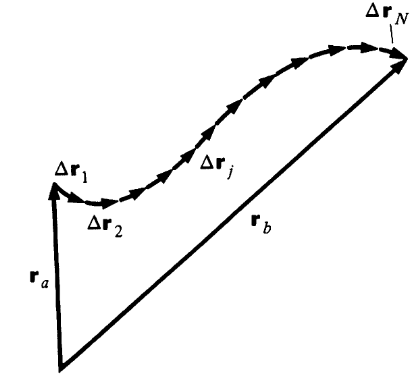
\includegraphics[scale=0.5]{lineint}
  \caption{Integral de línea}
  \label{fig:lineint}
\end{figure}
\end{frame}

Si $\Delta \mathbf{r}_j$ es suficientemente pequeño, el integrando del lado derecho de la ec.~\eqref{eq:flinea} puede escribirse como
\begin{align}
  \label{eq:dW}
  \mathbf{F}(\mathbf{r}_j)\cdot\Delta\mathbf{r}_j
\end{align}

Si $\Delta t$ es el tiempo que se tarda en atravesar un segmento, entonces
\begin{align}
  \Delta\mathbf{r}_j = \mathbf{r}(t_j+\Delta t)-\mathbf{r}(t_j)=\frac{\Delta\mathbf{r}}{\Delta t}\Delta t\,,
\end{align}
\begin{align}
  \int_C \mathbf{F}(\mathbf{r})\cdot\,d\mathbf{r}=&\lim_{\Delta t\to 0}\sum_{j=1}^N\mathbf{F}(\mathbf{r}_j)\cdot\frac{\Delta\mathbf{r}}{\Delta t}\Delta t\nonumber\\
=&\int_{t_a}^{t_b}\mathbf{F}(\mathbf{r}(t))\cdot\frac{d\mathbf{r(t)}}{dt}\,dt\,.
\end{align}
\begin{inprogress}
  Ejemplos de integrales de Línea para fuerzas constantes y centrales.
\end{inprogress}


\section{Ecuación de la trayectoria}

Aplicando el concepto de integral de línea a la ecuación de movimiento con masa constante
\begin{align}
\label{eq:trayectoria}
  \mathbf{F}(\mathbf{r})=&m\frac{d\mathbf{v}}{dt}\nonumber\\
  \int_C\mathbf{F}(\mathbf{r})\cdot d\mathbf{r}=&m\int_C\frac{d\mathbf{v}}{dt}\cdot d\mathbf{r}\nonumber\\
 \int_{t_a}^{t_b}\mathbf{F}(\mathbf{r})\cdot \frac{d\mathbf{r}}{dt}\,dt=&m\int_{t_a}^{t_b}\frac{d\mathbf{v}}{dt}\cdot \frac{d\mathbf{r}}{dt}\,dt\,.
\end{align}

Analicemos primero el caso del movimiento bajo una fuerza $F(x)$ en una dimensión. La ec.~\eqref{eq:trayectoria} queda
\begin{align}
  \label{eq:1dt}
 \int_{t_a}^{t_b}F(x)\frac{dx}{dt}\,dt=&m\int_{t_a}^{t_b}\frac{dv}{dt}\frac{dx}{dt}\,dt\nonumber\\\, 
 =&m\int_{t_a}^{t_b}\frac{dv}{dt}v\,dt\nonumber\\\, 
 =&m\int_{t_a}^{t_b}v\,\frac{dv}{dt}dt\,.
\end{align}
Realizando el cambio de variables
\begin{align}
  t\to&x(t) & t\to&v(t)\nonumber\\
 t_a\to& x(t_a)=x_a& t_a\to& v(t_a)=v_a\nonumber\\
 t_b\to& x(t_b)=x_b& t_b\to& v(t_b)=v_b\nonumber\\
 \frac{dx}{dt}dt\to& dx& \frac{dv}{dt}dt\to&dv\,,
\end{align}
y reemplazando en \eqref{eq:1dt}
\begin{align}
  \label{eq:1dtn}
 \int_{x_a}^{x_b}F\,{dx}=&m\int_{v_a}^{v_b}v\,{dv}\nonumber\\
 =&\left.\frac{1}{2}mv^2\right|_{v_a}^{v_b}\nonumber\\
=&\tfrac{1}{2}mv_b^2-\tfrac{1}{2}mv_a^2\,.
\end{align}
Definimos:
\begin{align}
  \label{eq:K}
  K\equiv&\frac{1}{2}m v^2\nonumber\\
  W_{a b}\equiv&\int_{x_a}^{x_b}F(x)dx\,,
\end{align}
donde $K$ es la \emph{energía cinética}, y $W_{a b}$ es el \emph{trabajo} hecho por la fuerza $F$ sobre la partícula a medida que ésta se mueve de $a$ a $b$. Entonces la ec.~(\ref{eq:1dtn}) queda
\begin{align}
    W_{ba}=K_b-K_a\,.
\end{align}




En el caso general de tres dimensiones, el lado derecho de la ec.~\eqref{eq:trayectoria} se puede evaluar directamente
\begin{align}
  \int_C\frac{d\mathbf{v}}{dt}\cdot d\mathbf{r}
 =&\lim_{\Delta t\to 0}\sum_{j=1}^N\frac{d\mathbf{v}}{dt}\cdot\frac{\Delta\mathbf{r}}{\Delta t}\Delta t\,.
\end{align}
Para un segmento suficientemente corto, $\mathbf{v}$ es aproximadamente constante. De aquí que $\Delta\mathbf{r}=\mathbf{v}\Delta t$, por consiguiente
\begin{align}
    \int_C\frac{d\mathbf{v}}{dt}\cdot d\mathbf{r}
    =&\int_{t_a}^{t_b}\frac{d\mathbf{v}}{dt}\cdot\mathbf{v}dt\nonumber\\
    =&\int_{t_a}^{t_b}\frac{1}{2}\left(\mathbf{v}\cdot\frac{d\mathbf{v}}{dt}+\frac{d\mathbf{v}}{dt}\cdot\mathbf{v}\right)dt\nonumber\\
    =&\int_{t_a}^{t_b}\frac{1}{2}\frac{d}{dt}\left(\mathbf{v}\cdot\mathbf{v}\right)dt\nonumber\\
    =&\int_{t_a}^{t_b}\frac{1}{2}\frac{d}{dt}(v^2)\,dt\,.
\end{align}
Como la antiderivada de $v^2$ es justamente $d(v^2)/dt$, entonces
\begin{align}
  \int_C\frac{d\mathbf{v}}{dt}\cdot d\mathbf{r}
  =&\int_{t_a}^{t_b}\frac{1}{2}\frac{d}{dt}(v^2)\,dt\nonumber\\
  =&\left.\frac{1}{2}v^2\right|_{t_a}^{t_b}\nonumber\\
  =&\tfrac{1}{2}v(t_b)^2-\tfrac{1}{2}v(t_a)^2\nonumber\\
  =&\tfrac{1}{2}v_b^2-\tfrac{1}{2}v_a^2\,.
\end{align}
y reemplazando en la ecuación para la trayectoria~\eqref{eq:trayectoria}
\begin{align}
  \label{eq:linev2}
    \int_C\mathbf{F}(\mathbf{r})\cdot d\mathbf{r}=&m\int_C\frac{d\mathbf{v}}{dt}\cdot d\mathbf{r}\nonumber\\
  =&\tfrac{1}{2}mv_b^2-\tfrac{1}{2}mv_a^2\,.
\end{align}

\section{Teorema de Trabajo-Energía}
El trabajo hecho por una fuerza $\mathbf{F}$ sobre una partícula que se mueve de $a$ hasta $b$, se define como
\begin{align}
  W_{ba}=\int_C\mathbf{F}\cdot d\mathbf{r}\,.
\end{align}
La ecuación (\ref{eq:linev2}) toma ahora la forma
\begin{align}
  \label{eq:tte}
  W_{ba}=K_b-K_a\,.
\end{align}
donde $K$ es la energía cinética de la partícula de masa $m$ y una rapidez $v$ y esta dada por la ec.~\eqref{eq:K},
\begin{align*}
  K=\tfrac{1}{2}m v^2\,.
\end{align*}



Para un sistema extendido
\begin{align}
  \int_C \mathbf{F}\cdot d\mathbf{R}=\tfrac{1}{2}M V_b^2-\tfrac{1}{2}M V_a^2\,,
\end{align}
donde $d\mathbf{R}=\mathbf{V}dt$ es el desplazamiento del centro de masa en un tiempo $t$.


\section{Cálculo del trabajo}
En el caso de movimiento en una dimensión
\begin{align*}
  \mathbf{F}=(F_x,0,0)
\end{align*}
la integral de línea se reduce a una integral normal
\begin{align*}
  \int_{\text{1-dim}}\mathbf{F}\cdot d\mathbf{R}=\int_{x_0}^{x}F_x(x)\,dx\,.
\end{align*}


\subsection{Fuerza gravitacional constante}
\begin{frame}
Considere el trabajo que tiene que realizar la fuerza gravitacional
para reducir la rapidez de una partícula que ha sido lanzada hacia
arriba con rapidez $v_0$ hasta una rapidez $v$. Tomando el origen de coordenadas en la superficie de la tierra, tenemos
\begin{align*}
  \mathbf{F}=&(0,-mg,0)\nonumber\\
  d\mathbf{r}=&(dx,dy,dz)\,.
\end{align*}
entonces
\begin{align*}
  W_{ba}=-mg\int_{y_0}^ydy=-mg(y-y_0)<0\,.
\end{align*}
y usando la ecuación (\ref{eq:linev2})
\begin{align}
  \label{eq:consrven}
  mgy_0-mgy=\tfrac{1}{2}m v^2-\tfrac{1}{2}m v_0^2\,,
\end{align}
\end{frame}
de donde
\begin{align*}
  v^2-v_0^2=-2g(y-y_0)\,,
\end{align*}
que corresponde a la ecuación de la trayectoria en la
ecuación~\eqref{eq:trayl}. De modo que la Segunda ley de Newton en la
forma del Teorema de trabajo y energía sirve para obtener directamente
la ecuación de la trayectoria.

Finalmente, podemos reescribir la ecuación~\eqref{eq:consrven} en la
forma
\begin{align}
  \tfrac{1}{2}m v_0^2+mgy_0=\tfrac{1}{2}m v^2+mgy\,.
\end{align}

\subsection{Trabajo realizado por la fuerza de fricción}
\begin{frame}
  Considere el trabajo realizado por la fuerza de fricción para reducir
la rapidez inicial de un cuerpo lanzado con rapidez inicial $v_0$
sobre una superficie horizontal con coeficiente de fricción dinámico
$\mu$, hasta una rapidez $v$. Tomando el origen de coordenadas en la
superficie, tenemos
\begin{align*}
  \mathbf{f}=&(-\mu m g,0,0)\nonumber\\
  d\mathbf{r}=&(dx,dy,dz)\,.
\end{align*}
entonces
\begin{align*}
  W_{ba}=-mg\int_{x_0}^x\,dx=-\mu mg(x-x_0)<0\,.
\end{align*}
y usando la ecuación (\ref{eq:linev2})
\begin{align*}
  \mu mgx_0-\mu mgx=\tfrac{1}{2}m v^2-\tfrac{1}{2}m v_0^2\,.
\end{align*}
\end{frame}
y
\begin{align}
x=x_0+\frac{v_0^2-v^2}{2\mu g}
\end{align}
La principal diferencia entre los dos movimientos estudiados es que
cuando la velocidad final es igual a cero, el movimiento bajo una
fuerza gravitacional constante continua (con la velocidad en sentido
opuesto), mientras que en el caso de fuerza de fricción el movimiento
se detiene completamente. Definiendo la energía potencial como
\begin{align*}
  U(y)=mg y\,,
\end{align*}
y la energía mecánica como
\begin{align*}
  E_{\text{mecánica}}=U(y)+\tfrac{1}{2}m v^2\,,
\end{align*}
podríamos explicar porque aparece la diferencia. Si asumimos que la
energía mecánica se conserva entonces la energía cinética se debe ir
convirtiendo en energía potencial para poder mantener la energía
mecánica constante. En el punto de máxima altura la energía mecánica
es sólo energía potencial y al siguiente instante la energía potencial
debe disminuir, es decir, el cuerpo debe comenzar a caer, para que la
energía potencial puede comenzar a generar de nuevo energía cinética. 

En el caso de la fuerza de fricción, la energía cinética es cero pero
no se ha convertido en ninguna otra forma de energía mecánica. Si
insistimos en la \emph{conservación de energía}, entonces
necesariamente la energía cinética se debe disipar en alguna otra
forma de energía que no puede usarse para continuar el movimiento del
bloque. Esta forma de energía se llama calor y se refleja en el
calentamiento (aumento de temperatura) entre las
superficies. Aceptando este postulado podríamos medir el calor en
unidades de energía mecánica. 

La unidad de trabajo y energía en el SI es el joule ($\si{\joule}$):
\begin{align}
  \SI{1}{\joule}=\SI{1}{\kilo\gram\metre^2\per\second^2}\,.
\end{align}
La unidad de trabajo y energía en el sistema cgs es el ergio ($\text{erg}$):
\begin{align}
  1\ \text{erg}=&\SI{1}{\gram\centi\meter^2\per\second^2}\nonumber\\
=&10^{-7}\si{\joule}\,.
\end{align}

Precisamente fue el físico Británico James Prescott Joule el primer en
apreciar que el calor en si mismo representa una forma de energía. A
través de una serie de experimentos meticulosos sobre le calentamiento
del agua por una rueda de paletas movidas por un cuerpo cayendo,
mostró que la perdida de la energía mecánica por fricción estaba
acompañada por la aparición de una cantidad de energía equivalente por
fricción. Joule concluyó que el calor es una forma de energía y que la
suma de la energía mecánica y la energía calórica de un sistema es
conservada.

Otra diferencia importante entre los dos sistemas es que el trabajo
realizado por la fuerza gravitacional para el cambio de altura entre
$y_0$ y $y$ es independiente de si el movimiento es puramente vertical
o parabólico. Sin embargo, para el cuerpo desplazándose sobre la misma
distancia en $x$ sobre una superficie con fricción pero siguiendo una
trayectoria curva, la fuerza de fricción realiza un trabajo mayor y
disipa más calor.





\section{Fuerzas conservativas}
En la naturaleza hay ciertas fuerzas, como la de la gravedad por
ejemplo, que tienen una propiedad muy especial llamada
\emph{conservativa}. Si calculamos el trabajo hecho por una fuerza al
mover un objeto de un punto a otro a lo largo de una trayectoria
curvada, en general (como en el caso de la fuerza de fricción) el
trabajo depende de la curva, pero en algunos casos especiales no. Si
el trabajo no depende de la curva, decimos que la fuerza es
conservativa. En otras palabras, si la integral de línea de la fuerza
veces la distancia para ir de la posición 1 a 2 es calculada lo largo
de una trayectoria $A$ y entonces a lo largo de $B$ y se obtiene lo
mismo, y si es cierto para éste par de números a lo largo de
\emph{todas las curvas}, y si pasa sin importar el par de números que
usemos, entonces decimos que la fuerza es conservativa. En tales casos
el trabajo se puede calcular de una manera simple, y podemos dar una
fórmula para el resultado.

Sea el trabajo de ir de un punto $P$ a otro punto del espacio: $-U(x,y,z)$, entonces si la fuerza es conservativa (manteniendo presente que tenemos integrales de línea)

\begin{minipage}{0.5\linewidth}
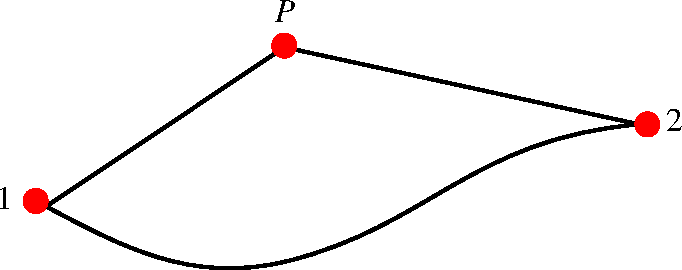
\includegraphics[scale=0.7]{paths}  
\end{minipage}
\begin{minipage}{0.5\linewidth}
  \begin{align}
  \int_1^2 \mathbf{F}\cdot d\mathbf{r}
  =&\int_1^P \mathbf{F}\cdot d\mathbf{r}+\int_P^2 \mathbf{F}\cdot d\mathbf{r}\nonumber\\
  =&-\int_P^1 \mathbf{F}\cdot d\mathbf{r}+\int_P^2 \mathbf{F}\cdot d\mathbf{r}\nonumber\\
  =&-(-U(x_1,y_1,z_1))-U(x_2,y_2,z_2)\nonumber\\
  =&U(x_1,y_1,z_1)-U(x_2,y_2,z_2)\nonumber\\
  =&U(\mathbf{r}_1)-U(\mathbf{r}_2)\,.
\end{align}
\end{minipage}

La cantidad $U(\mathbf{r}_1)-U(\mathbf{r}_2)$ es llamada el cambio en \emph{energía potencial}, y llamaremos $U$ la energía potencial.

Para el caso de fuerzas conservativas, la ec.~(\ref{eq:tte}) queda
\begin{align}
  U(\mathbf{r_a})-U(\mathbf{r_b})=&K_b-K_a\nonumber\\
  K_a+U(\mathbf{r_a})=&K_b+U(\mathbf{r_b})\,,
\end{align}
Como esto se mantiene para cualquier par de puntos $\mathbf{r}_a$ y $\mathbf{r}_b$, entonces
\begin{align}
  E\equiv K+U=\text{constante}\,.
\end{align}
La constante $E$ es llamada la \emph{energía mecánica} de la partícula, o de forma menos precisa, la energía total de la partícula. 

La Ley de Convervación de la Energía Mecánica es una consecuencia de la homogeneidad del tiempo.

Supongamos que tenemos un sistema unidimensional, en el cual la fuerza $F(x)$ es conservativa, de modo que la diferencia de energía potencial es
\begin{align}
  U_b-U_a=&-\int_C \mathbf{F}\cdot d\mathbf{r}\nonumber\\ 
  =&-\int_{t_a}^{t_b} \mathbf{F}\cdot \frac{d\mathbf{r}}{dt}dt\nonumber\\ 
  =&-\int_{t_a}^{t_b} F\frac{dx}{dt}dt\nonumber\\ 
  =&-\int_{x_a}^{x_b} F\,{dx}\,.
\end{align}
Consideremos el cambio en la energía potencial $\Delta U$ a medida que la partícula se mueve desde algún punto $x$ a $x+\Delta x$
\begin{align}
  U(x+\Delta x)-U(x)\equiv&\Delta U\nonumber\\
  =&-\int_x^{x+\Delta x}F(x)\,dx\nonumber\\
\approx &-F(x)\int_x^{x+\Delta x}\,dx\nonumber\\
=&-F(x)(x+\Delta x-x)\nonumber\\
=&-F(x)\Delta x\,,
\end{align}
o
\begin{align}
  F(x)\approx -\frac{\Delta U}{\Delta x}
\end{align}
en el límite $\Delta x\to 0$ estaríamos tentados a escribir $dU/dx$, sin embargo es más conveniente hacer explícito que la variación es sólo sobre $x$ usando la notación
\begin{align}
  F(x)= -\frac{\partial U}{\partial x}
\end{align}
definida como la derivada parcial por los matemáticos. Note entonces que en el caso unidimensional la energía potencial es justamente la antiderivada de $F(x)$

En el caso de una fuerza conservativa en tres dimensiones siempre podemos escoger una trayectoria para ir del punto 1 al punto 2 de tal forma que se mantengan dos de las direcciones constantes. A lo largo de cada dirección podemos aplicar el método anterior variando $U$ sólo en la dirección relevante. Por ejemplo,
para una fuerza en tres dimensiones
\begin{align}
  \mathbf{F}=F_x\hat{\mathbf{i}}+F_y\hat{\mathbf{j}}+F_y\hat{\mathbf{k}}\,,
\end{align}
si escogemos una trayectoria a lo largo de $x$ llegaríamos al resultado
\begin{align}
  F_x=&-\lim_{\Delta x\to 0} \frac{U(x+\Delta x,y,z)}{\Delta x}\nonumber\\
  =&-\left.\frac{\partial U}{\partial x}\right|_{yz}\,.
\end{align}
donde la parte de ``$|_{yz}$'' hace explícito que la variación se hace manteniendo las direcciones $y$ y $z$ constantes. En adelantes usaremos la notación de derivadas parciales sin explicitar la variables que se dejan constantes pues se sobreentiende del contexto.

Por un método completamente análogo para las otras direcciones, se llega al sistema de ecuaciones. 

\begin{align}
  F_x=& -\frac{\partial U}{\partial x}\nonumber\\
   F_y=& -\frac{\partial U}{\partial y}\nonumber\\
   F_z=& -\frac{\partial U}{\partial z}\,.
\end{align}
O en notación vectorial
\begin{align}
 \mathbf{F}=F_x\hat{\mathbf{i}}+F_y\hat{\mathbf{j}}+F_z\hat{\mathbf{k}}
=&-\left(\hat{\mathbf{i}}\frac{\partial U}{\partial x}
+\hat{\mathbf{j}}\frac{\partial U}{\partial y}
+\hat{\mathbf{k}}\frac{\partial U}{\partial z}\right)\nonumber\\
=&-\left(\hat{\mathbf{i}}\frac{\partial }{\partial x}
+\hat{\mathbf{j}}\frac{\partial }{\partial y}
+\hat{\mathbf{k}}\frac{\partial }{\partial z}
\right)U\nonumber\\
\mathbf{F}\equiv& -\boldsymbol{\nabla}U\,.
\end{align}
El operador
\begin{align}
\boldsymbol{\nabla}\equiv \hat{\mathbf{i}}\frac{\partial }{\partial x}
+\hat{\mathbf{j}}\frac{\partial }{\partial y}
+\hat{\mathbf{k}}\frac{\partial }{\partial z}
\end{align}
se llama \emph{gradiente} y convierte una función escalar de varias variables en una función vectorial. De éste modo para un campo conservativo, la integral de línea entre $a$ y $b$ se puede evaluar dando como resultado:
\begin{align}
  \int_C\mathbf{F}\cdot d\mathbf{r}=U(\mathbf{r}_a)-U(\mathbf{r}_b)
\end{align}
Generalizando el caso de la integración normal en una variable,
$-U(\mathbf{r})$ se podría ver como el ``antigradiente'' de
$\mathbf{F}$. El concepto de fuerza conservativa tiene su contraparte
matemática para establecer teoremas de integrabilidad de funciones de
varias variables. Para las fuerzas conservativas el campo generado por
el vector de fuerza se puede conocer a partir del \emph{gradiente} de
variaciones de una función escalar llamada el potencial.

\section{Conservación de la energía}
Las fuerzas fundamentales, o más estrictamente, las interacciones
fundamentes conocidas en la naturaleza, son todas conservativas. Como
consecuencia, la energía total de un sistema de partículas se debe
conservar. Estas interacciones fundamentales pueden generar algunas
fuerzas remanentes como la fricción que aparentemente es no
conservativa: el trabajo para arrastrar un objeto entre un par de
puntos por diferentes caminos con fricción, depende de la trayectoria
que se siga el objeto. Sin embargo, la fricción es una herramienta
para parametrizar detalles de las interacciones interatómicas las
cuales si son conservativas. La energía cinética y los diferentes
potenciales interatómicos cambian con el movimiento de un cuerpo sobre una
superficie con fricción. Estos procesos se reflejan en el calor
disipado por el cuerpo mientras se mueve sobre la superficie. En
términos modernos la temperatura de un material es una consecuencia
de la energía cinética y potencial de sus componentes. Si tenemos en
cuenta la energía mecánica del sistema y las perdidas por calor, la
energía total del sistema se debe conservar, aunque en la practica
resulte extremadamente complicado calcular el calor generado por las
interacciones conservativas entre los átomos y moléculas del sistema.

Como dijimos antes, Joule fue el primer en apreciar que
el calor en si mismo representa una forma de energía. 
En nuestros días tenemos un conocimiento más detallado de la energía
calórica que la que tenía Joule. Sabemos que los sólidos están
compuestos por átomos mantenidos juntos por fuertes interacciones
interatómicas. Cada átomo puede oscilar sobre su posición de
equilibrio y tiene una energía mecánica en forma de energías cinéticas
y potenciales provenientes de interacciones conservativas. A medida
que el sólido se calienta, la amplitud de las oscilaciones se
incrementa y la energía promedio de cada átomo se vuelve mayor. La
energía calórica de un sólido es la energía mecánica de las
vibraciones aleatorias de los átomos.
   

\section{Ejemplos de energía potencial}

\subsection{Energía potencial de un campo de fuerza uniforme}
\begin{align}
  U(h)=mgh\,,
\end{align}
donde $h$ es la altura desde el suelo.

\begin{itemize}
\item[\textbf{Ejemplo:}] \textbf{Caída libre}\\
Si $\mathbf{F}=-mg\hat{\mathbf{j}}$, $d\mathbf{r}=\hat{\mathbf{j}}dy$ tenemos
\begin{align}
\label{eq:12e}
  \tfrac{1}{2}mv_b^2-\tfrac{1}{2}mv_a^2=&\int\mathbf{F}\cdot d\mathbf{r}\nonumber\\
  =&-mg \int_{y_a}^{y_b}\, dy\nonumber\\
  \tfrac{1}{2}mv_b^2-\tfrac{1}{2}mv_a^2=&-gm(y_b-y_a)\,.
\end{align}

De esta forma hemos obtenido directamente la ecuación de la trayectoria para caída libre \eqref{eq:trayl}
\begin{align}
  \tfrac{1}{2}v_b^2-\tfrac{1}{2}v_a^2=&-g(y_b-y_a)\,.
\end{align}

En términos de conservación de la energía mecánica, la ec~(\ref{eq:12e}) también puede escribirse como:
\begin{align}
  \tfrac{1}{2}v_a^2+mgy_a=&\tfrac{1}{2}mv_b^2+mgy_b
\end{align}


Para encontrar la altura máxima de un cuerpo lanzado horizontalmente hacia arriba desde la superficie de la tierra, con rapidez inicial $v_0$, igualamos la energía cinética incial con la energía potencial final:
\begin{align}
  \frac{1}{2}mv_0^2=mgy_{\text{max}}\,,
\end{align}
de donde
\begin{align}
  y_{\text{max}}=\frac{v_0^2}{2g}\,.
\end{align}

\end{itemize}


\ejemplo{}
\label{ex:polea}


 Un cuerpo de masa $m_2$ se desliza desde el
  reposo sobre una mesa sin fricción debido al peso de un bloque de
  masa $m_1>m_2$ que cae desde una altura $y_0$ y con el cual está
  conectado a través de una polea ideal. Ver figura~\ref{fig:poleaideale}

La conservación de energía se aplica al sistema completo:
\begin{align}
  \text{Energía mecánica inicial de los dos bloques}=
\text{Energía mecánica final de los dos bloques}
\end{align}
Como los dos bloques se mueven con la misma rapidez $v$, y asumiendo
sin perdida de generalidad que la altura final del bloque 1 es cero,
tenemos (asumiendo que la altura de la mesa es $h$)

\begin{frame}
  \begin{figure}
    \centering
    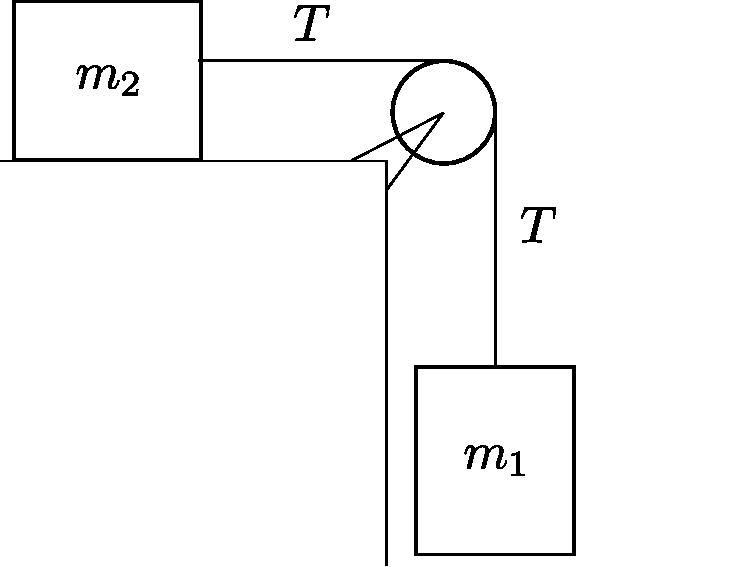
\includegraphics[scale=0.5]{poleaideal}
    \caption{Polea ideal}
    \label{fig:poleaideale}
  \end{figure}
\end{frame}

\begin{frame}
\begin{align*}
  m_1gy_0+\cancel{m_2gh}=&\tfrac{1}{2}m_1 v^2+\tfrac{1}{2}m_2 v^2+\cancel{m_2gh}\phantom{\color{red}+Q}\nonumber\\
 \phantom{\color{red}-\mu m_2 g y_0+}m_1gy_0=&\tfrac{1}{2}m_1 v^2+\tfrac{1}{2}m_2 v^2
  =\tfrac{1}{2}(m_1+m_2) v^2\,,
\end{align*}
despejando $v$, obtenemos
\begin{align*}
  v^2=2gy_0\,\frac{m_1\phantom{\color{red}-\mu m_2}}{m_1+m_2}\,.
\end{align*}
Para un movimiento bajo aceleración constante, y teniendo en cuenta que la altura final es cero
\begin{align*}
  0=&y_0-\tfrac{1}{2}a\Delta t^2\,,&
  v=&-a\Delta t\,,
\end{align*}
tenemos, de la última ecuación
\begin{align*}
  a^2 \Delta t^2=v^2
  =&2gy_0\,\frac{m_1\phantom{\color{red}-\mu m_2}}{m_1+m_2}\nonumber\\
  a^{\cancel{2}} \cancel{\Delta t^2}=&\frac{2}{2}g\,\cancel{a\Delta t^2}\,\frac{m_1\phantom{\color{red}-\mu m_2}}{m_1+m_2}\,,
\end{align*}
de donde
\begin{align}
\label{eq:acelfin}
  a=g\,\frac{m_1\phantom{\color{red}-\mu m_2}}{m_1+m_2}\,,
\end{align}
\end{frame}
que coincide con el resultado expresado en la ecuación \eqref{eq:polea} cuando $\mu=0$.


Usando directamente las leyes de Newton, como hicimos en los problemas resueltos del capítulo de dinámica
\begin{align}
  T=&m_2 a\nonumber\\
m_1g-T=&m_1 a\,,
\end{align}
donde $T$ es la tensión de la cuerda. 


\begin{inprogress}
  \begin{itemize}
  \item[\textbf{Ejemplo:}] \textbf{Energía potencial de un campo de fuerza uniforme}
  \end{itemize}
\end{inprogress}

\begin{inprogress}
  \begin{itemize}
  \item[\textbf{Ejemplo:}] \textbf{El péndulo invertido}
  \end{itemize}
\end{inprogress}


\section{Fuerzas no conservativas}
La fuerza total se puede escribir como
\begin{align}
  \mathbf{F}=\mathbf{F}^{\text{c}}+\mathbf{F}^{\text{nc}}
\end{align}
donde $\mathbf{F}^{\text{c}}$ y $\mathbf{F}^{\text{nc}}$ son las fuerzas conservativas y no conservativas respectivamente. El trabajo total es
\begin{align}
  W_{ba}^{\text{total}}=&\int_C \mathbf{F}\cdot d\mathbf{r}\nonumber\\
=&\int_C \mathbf{F}^{\text{c}}\cdot d\mathbf{r}+\int_C \mathbf{F}^{\text{nc}}\cdot d\mathbf{r}\nonumber\\
=-U_b+U_a+W_{ba}^{\text{nc}}\,.
\end{align}
Aquí $U$ es la energía potencial asociada con las fuerza conservativa y $W_{ab}^{\text{nc}}$ es el trabajo hecho por la fuerza no conservativa. El teorema de trabajo-energía, $W_{ba}^{\text{total}}=K_b-K_a$, ahora toma la forma
\begin{align}
  -U_b+U_a+W_{ba}^{\text{nc}}=K_b-K_a\,,
\end{align}
ó
\begin{align}
  K_b+U_b=K_a+U_a+W_{ba}^{\text{nc}}\,.
\end{align}
Si definimos la energía mecánica por
\begin{align}
  E=K+U\,,
\end{align}
tenemos
\begin{align}
  E_b-E_a=W_{ba}^{\text{nc}}\,.
\end{align}

Si definimos $Q=-W_{ab}$ como la energía disipada: la diferencia entre
la energía mecánica inicial y final
\begin{align}
  E_a=&E_b-W_{ba}^{\text{nc}}\nonumber\\
   E_a=&E_b+Q.
\end{align}
En el caso por ejemplo de la un movimiento en presencia de una fuerza
no conservativa como la fricción, $Q$ corresponde a la energía
disipada en forma de calor.

En el caso del ejemplo asociado a la figura~\ref{fig:poleaideale}, si consideramos que entre las dos superficies hay fuerza fricción, esta realiza un trabajo sobre el bloque $m_2$ que se disipa en calor $Q$, a medida que el cuerpo de masa $m_1$ cae una distancia $y_0$. El calor disipado esta dado por
\begin{align*}
    {\color{red}Q}=-W_{ba}=&\int_C \mathbf{F}\cdot d\mathbf{r}\nonumber\\
=&\int_C
\begin{pmatrix}
  -\mu m_2g,&0,&0
\end{pmatrix}\cdot
\begin{pmatrix}
dx,&dy,&dz  
\end{pmatrix}\nonumber\\
=&-(-\mu m_2 g)\int_0^{y_0}dx\nonumber\\
&={\color{red}\mu m_2g y_0\,,}
\end{align*}
donde $\mu$, es el coeficiente de fricción y donde hemos usado la
ligadura consistente en que la distancia vertical recorrida es la
misma que la distancia horizontal, pues la cuerda es ideal.
Repitiendo los pasos que dieron lugar a la ec.~\eqref{eq:acelfin}


\begin{frame}
\begin{align*}
  m_1gy_0+\cancel{m_2gh}=&\tfrac{1}{2}m_1 v^2+\tfrac{1}{2}m_2 v^2+\cancel{m_2gh}{\color{red}+Q}\nonumber\\
 {\color{red}-\mu m_2 g y_0+}m_1gy_0=&\tfrac{1}{2}m_1 v^2+\tfrac{1}{2}m_2 v^2
  =\tfrac{1}{2}(m_1+m_2) v^2\,,
\end{align*}
despejando $v$, obtenemos
\begin{align*}
  v^2=2gy_0\,\frac{m_1{\color{red}-\mu m_2}}{m_1+m_2}\,.
\end{align*}
Para un movimiento bajo aceleración constante, y teniendo en cuenta que la altura final es cero
\begin{align*}
  0=&y_0-\tfrac{1}{2}a\Delta t^2\,,&
  v=&-a\Delta t\,,
\end{align*}
tenemos, de la última ecuación
\begin{align*}
  a^2 \Delta t^2=v^2
  =&2gy_0\,\frac{m_1{\color{red}-\mu m_2}}{m_1+m_2}\nonumber\\
  a^{\cancel{2}} \cancel{\Delta t^2}=&\frac{2}{2}g\,\cancel{a\Delta t^2}\,\frac{m_1{\color{red}-\mu m_2}}{m_1+m_2}\,,
\end{align*}
de donde
\begin{align}
\label{eq:acelfinmu}
  a=g\,\frac{m_1{\color{red}-\mu m_2}}{m_1+m_2}
\end{align}

\end{frame}

\noindent
que coincide exactamente con el resultado obtenido en la ecuación \eqref{eq:polea} utilizando las ecuaciones de la dinámica. 

\begin{frame}
  \begin{block}{Recomendación}
    \emph{Siempre que pueda, resuelva los problemas por dos métodos diferentes y compruebe que obtiene la misma respuesta!}
    \begin{center}
          \begin{tabular}{cc}
      Ecuaciones de movimiento & Teorema trabajo y energía\\
      $\displaystyle a=g\,\frac{m_1{\color{red}-\mu m_2}}{m_1+m_2}$&
      $\displaystyle a=g\,\frac{m_1{\color{red}-\mu m_2}}{m_1+m_2}$\\
    \end{tabular}
    \end{center}
  \end{block}
\end{frame}

\begin{inprogress}
  \begin{itemize}
  \item[\textbf{Ejemplo:}] \textbf{Bloque deslizándose por un plano
      inclinado (Ejemplo 4.17 de Klepner)}\\
  \end{itemize}
\end{inprogress}


\section{Energía potencial de un resorte}
Por sencillez consideremos el caso de un resorte que se mueve a lo largo del eje $x$, como se muestra en la figura~\ref{fig:resorte}. Para una elongación $x-x_0$ a partir de su posición de equilibrio $x_0$ la fuerza está dada por la Ley de Hooke
\begin{align}
  \mathbf{F}=-k(x-x_0)\hat{\mathbf{i}}\,.
\end{align}
\begin{frame}
  \begin{figure}
    \centering
%\only<1>%
{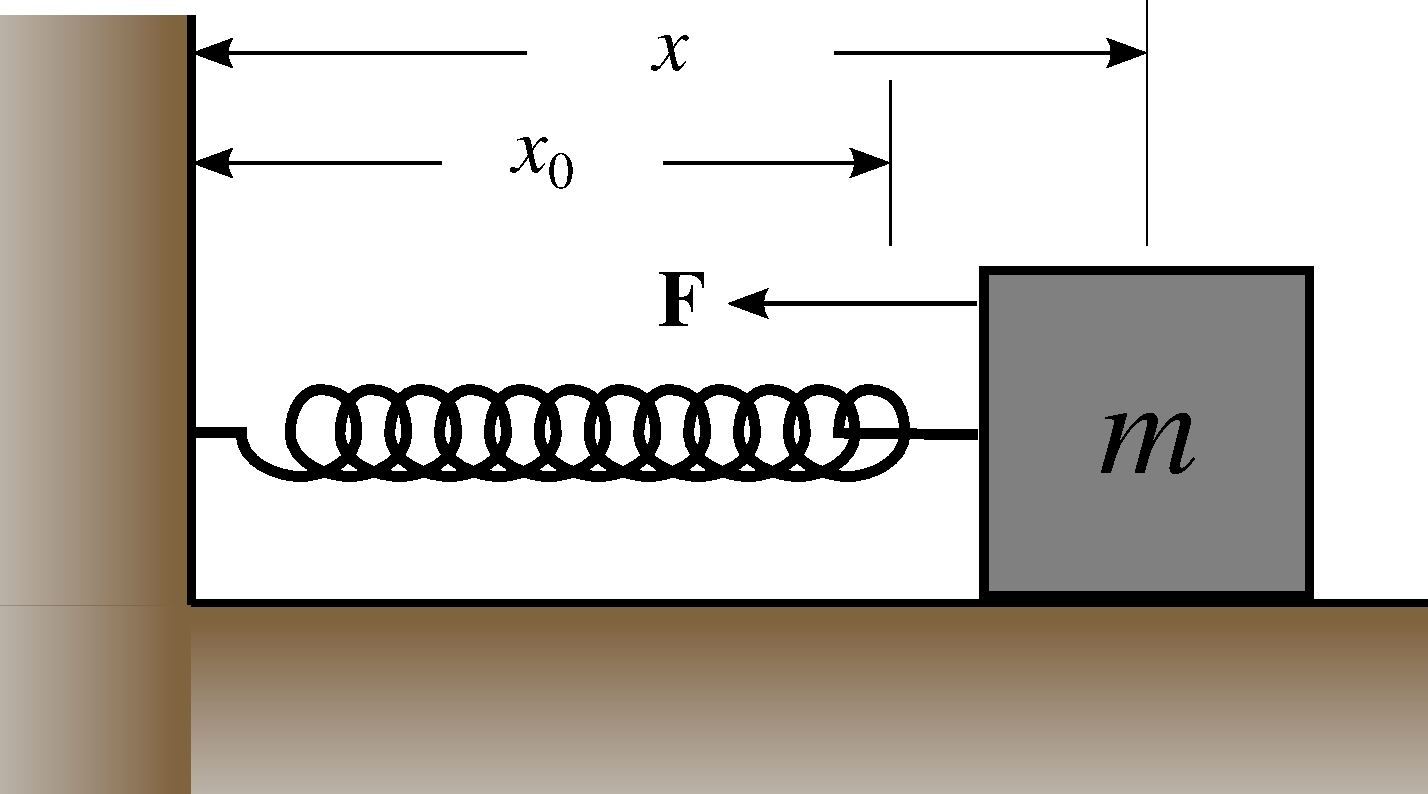
\includegraphics[scale=0.5]{resorte1}}
%\only<2>{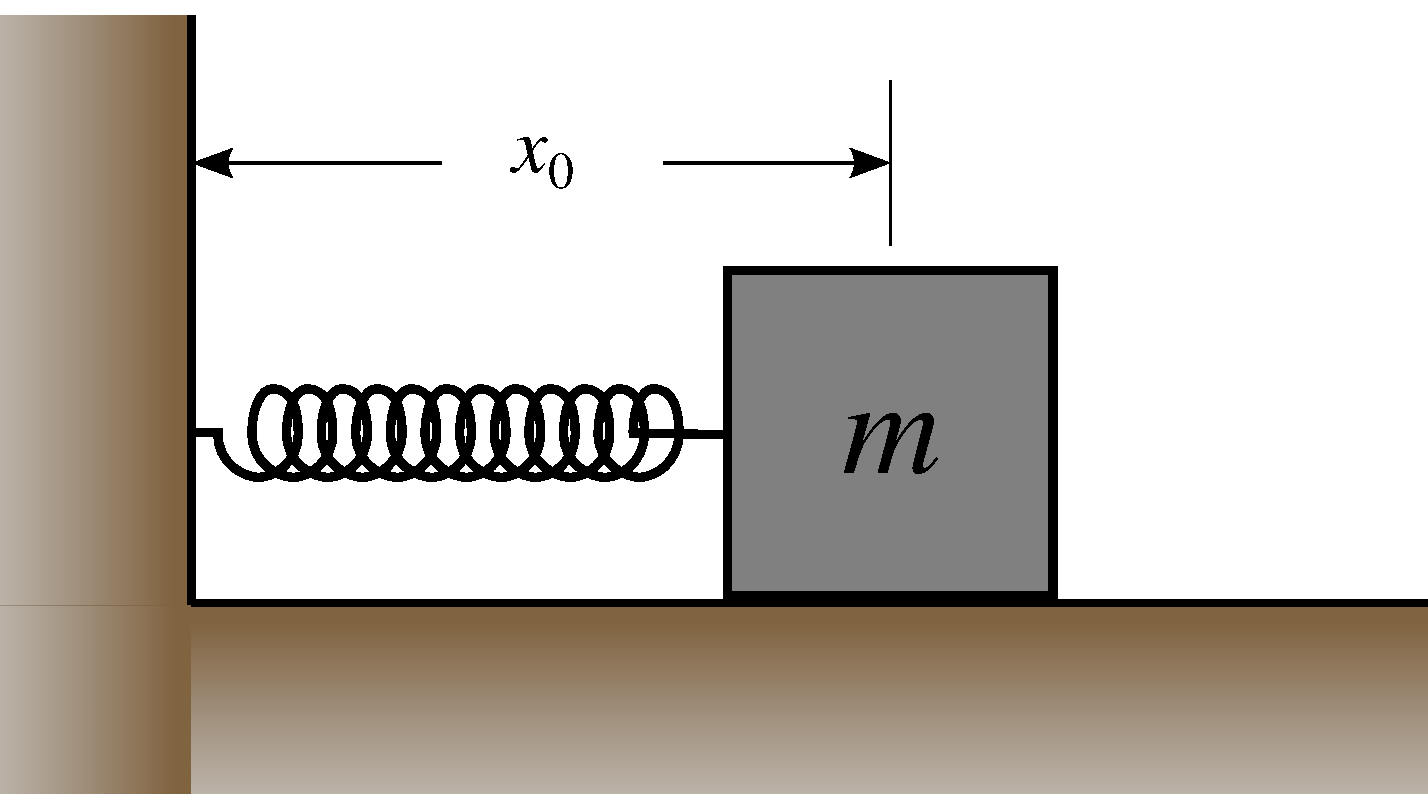
\includegraphics[scale=0.5]{resorte2}}%
%\only<3>{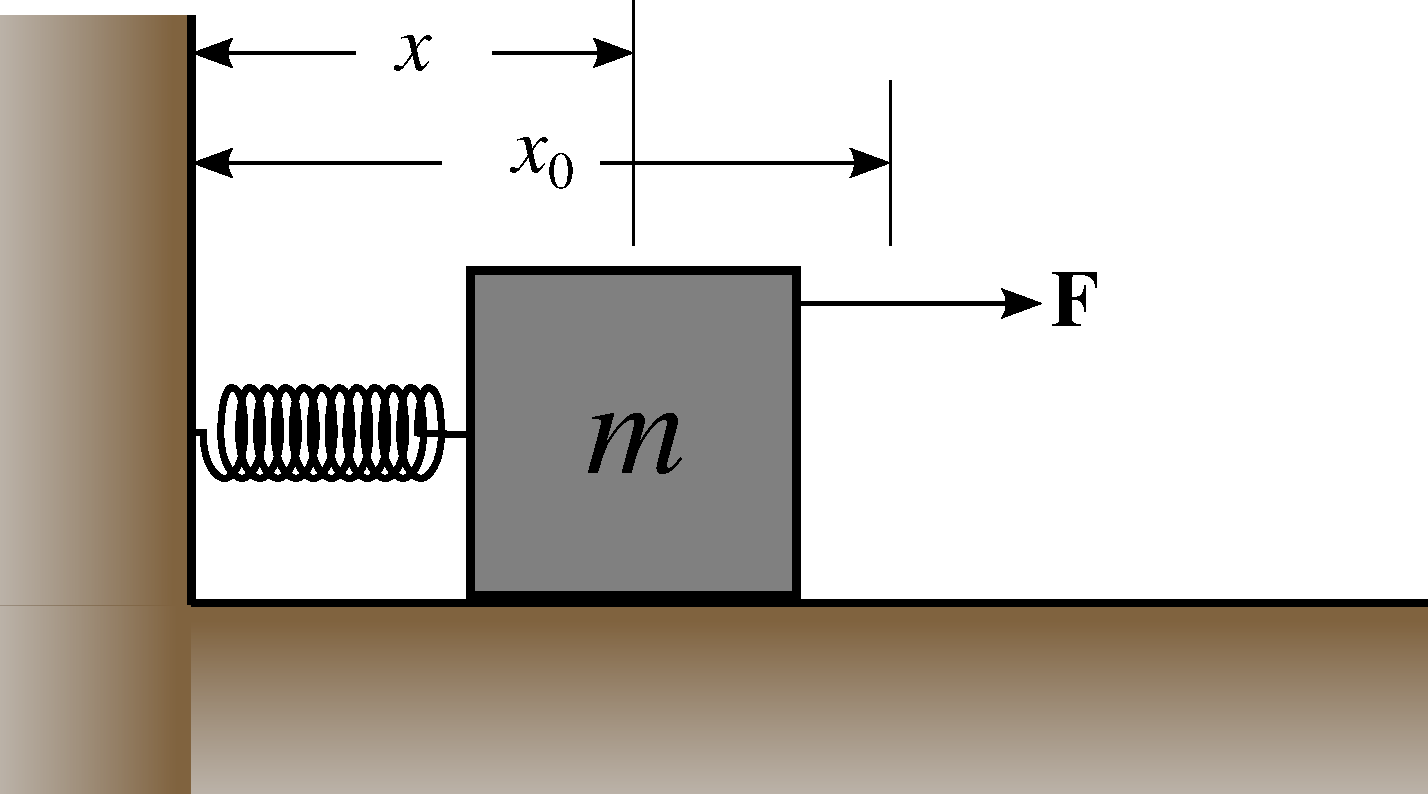
\includegraphics[scale=0.5]{resorte3}}%
    \caption{Resorte (Adaptado de Wikipedia)}
    \label{fig:resorte}
  \end{figure}
\end{frame}

El trabajo para ir de $a$ a $b$ es
\begin{align}
  W_{ab}=&\int \mathbf{F}\cdot d\mathbf{r}\nonumber\\
  =&\int_{x_a}^{x_b} Fdx\nonumber\\
  =&-k\int_{x_a}^{x_b} (x-x_0)dx\nonumber\\
  =&-\tfrac{1}{2}k \left.
    (x-x_0)^2\right|_{x_0}^x\nonumber\\
  =&-\tfrac{1}{2}k (x-x_0)^2+0\nonumber\\
  =&+0+C-(\tfrac{1}{2}k (x-x_0)^2+C)\nonumber\\
  =&U(x_0)-U(x)\,.
\end{align}
Y viceversa: de la siguiente energía potencial para el resorte,
\begin{align}
  U(x)=&\tfrac{1}{2}k{(x-x_0)^2}+C& C=&\text{contante}\,,
\end{align}
se puede obtener la fuerza conservativa
\begin{align}
  \mathbf{F}=-\frac{\partial}{\partial x}U(x)\hat{\mathbf{i}}
=&\left(
-\frac{2}{2}k(x-x_0)\frac{\partial}{\partial x}(x-x_0)+0
\right)\hat{\mathbf{i}}\nonumber\\
=&-k(x-x_0)\hat{\mathbf{i}}\,.
\end{align}

Por convención escogemos que la energía potencial sea cero en la posición de equilibrio:
\begin{align}
  U(x_0)=0=&\tfrac{1}{2}k{(x_0-x_0)^2}+C\nonumber\\
  0=&C\,,
\end{align}
de modo que la energía potencial para el resorte es
\begin{align}
  U(x)=&\tfrac{1}{2}k{(x-x_0)^2}\,.
\end{align}

\ejemplo{}
\label{ex:resorte}

En $t=0$ una masa atada a un resorte sobre
una superficie horizontal sin fricción, es
liberada desde el reposo a una distancia $x_i$ desde la posición de
equilibrio de un resorte. Encuentre la posición de la masa en
  cualquier tiempo posterior. Asumamos sin perdida de generalidad que
  la posición de equilibrio del resorte se encuentra en $x_0=0$

Usando la conservación de la Energía Mecánica:
\begin{align}
  K_i+U_i=&K_f+U_f\nonumber\\
 \tfrac{1}{2}kx_i^2=&\tfrac{1}{2}m v^2+\tfrac{1}{2}kx^2\nonumber\\
 kx_i^2=&m v^2+kx^2\,,
\end{align}
despejando $v$:
\begin{align}
  v=\sqrt{\frac{k}{m}}\sqrt{x_i^2-x^2}
\end{align}
note que la conservación de energía implica que $x\le x_i$. Entonces
\begin{align}
  \frac{dx}{dt}=\sqrt{\frac{k}{m}}\sqrt{x_i^2-x^2}\,.
\end{align}
Reorganizando términos
\begin{align}
  \label{eq:intosc}
  \frac{dx}{\sqrt{x_i^2-x^2}}=\omega dt\,,
\end{align}
donde hemos definido la frecuencia angular $\omega$ como:
\begin{align}
  \omega\equiv \sqrt{\frac{k}{m}}\,.
\end{align}
Integrando \eqref{eq:intosc}
\begin{align}
  \label{eq:intosc}
  \int_{x_i}^x\frac{dx}{\sqrt{x_i^2-x^2}}=\omega\int_0^t dt\,,
\end{align}
\begin{align}
\left.\sin^{-1}\left(\frac{x}{x_i}  \right)\right|_{x_i}^x=&\omega t\nonumber\\
\sin^{-1}\left(\frac{x}{x_i} \right)-\sin^{-1}\left(1\right)=&\omega t\nonumber\\
\sin^{-1}\left(\frac{x}{x_i} \right)-\frac{\pi}{2}=&\omega t\,,
\end{align}
despejando $x$, tenemos
\begin{align}
  x=x_i\sin\left(\omega t +\frac{\pi}{2}\right)
\end{align}
o
\begin{align}
  x=x_i\cos(\omega t)
\end{align}

  
%\left(  \right)


\begin{inprogress}
  \subsection{Estabilidad}

\section{Diagramas de energía}

\section{Oscilaciones pequeñas en un sistema ligado}

\end{inprogress}


  
\section{Potencia}
Potencia es la tasa de cambio del trabajo realizado. Si una fuerza $\mathbf{F}$ actúa en un cuerpo que sufre un desplazamiento $\Delta\mathbf{r}$, tenemos que el trabajo en dicho segmento es de la ec.\eqref{eq:dW}
\begin{align}
  \Delta W_j=\mathbf{F}(\mathbf{r}_j)\cdot \Delta \mathbf{r}_j\,.
\end{align}
en el límite $\Delta t\to 0$
\begin{align}
  dW=\mathbf{F}\cdot d\mathbf{r}\,.
\end{align}
Definimos la potencia desarrollada por la fuerza como
\begin{align}
  P=\frac{dW}{dt}=&\mathbf{F}\cdot \frac{d\mathbf{r}}{dt}\nonumber\\
=&\mathbf{F}\cdot \mathbf{v}\,.
\end{align}
La unidad de potencia en el sistema SI es el watt (W):
\begin{align}
  \SI{1}{\watt}=\SI{1}{\joule\per\second}\,.
\end{align}
La relación entre un caballo de fuerza y el watt es
\begin{align}
  1\;\text{hp}\approx \SI{746}{\watt}\,.
\end{align}
\example{} 
En la factura eléctrica se cobra la energía consumida al
mes.  El joule es una unidad demasiado pequeña, lo que obligaría a
emplear cifras demasiado grandes, por eso es conveniente reescribirlo
en potencia mayores. Note que
\begin{align}
  \SI{1}{\joule}=\si{\watt\second}\,.
\end{align}
De acuerdo a esto, pase a Joules las siguientes cantidades de energía
\begin{enumerate}
\item El $\si{\kilo\watt\hour}$ usado para medir el consumo electríco.
\item Los $\SI{75}{\giga\watt\hour}$ que consume el metro de Medellín en un año. 
%Si toda esa energía se pudiese convertir en energía cinética 
\end{enumerate}
\begin{align*}
  \SI{1}{\kilo\watt\hour}=&\SI{1000}{\watt}\cdot \SI{3600}{\second}\nonumber\\
  =&1000\frac{\si{\joule}}{\si{\second}}\cdot \SI{3600}{\second}\nonumber\\
  =&\SI{3600000}{\joule} \,.
\end{align*}

\begin{align*}
  \SI{75}{\giga\watt\hour}=&75\times 10^9\si{\watt}\cdot \SI{3600}{\second}\nonumber\\
  =&2.7\times 10^{14}\si{\joule}\,.
\end{align*}



\section{Colisiones}
Un sistema de dos partículas interaccionando en ausencia de fuerzas externas conserva el momentum total, de modo que
\begin{align}
\label{eq:consmom}
  \mathbf{P}_i=&\mathbf{P}_f\nonumber\\
m_1\mathbf{v}_1+m_2\mathbf{v}_2=&m_1\mathbf{v}'_1+m_2\mathbf{v}'_2\,.
\end{align}


\subsection{Colisiones elásticas}
Una colisión en la cual la energía la energía cinética no cambia 
es llamada una \emph{colisión elástica}. Una colisión es elástica si
las fuerzas de interacción son conservativas, como por ejemplo la
interacción entre dos bloques que se deslizan sin fricción
interaccionando a través de resortes, como se ilustra en la
figura~\ref{fig:colisionelastica}.


\begin{frame}
En tal caso, la conservación de la energía cinética da lugar a la ecuación
\begin{equation}
\label{eq:E2}
  m_1 v^2_1 + m_2 v^2_2 = m_1 {v'}^2_1 + m_2 {v'}^2_2\,.
\end{equation}

Si la colisión se desarrolla en una sola dimensión, la ec.~\eqref{eq:consmom} se reduce a 
\begin{equation}\label{eq:E1}
  m_1 v_1 + m_2 v_2 = m_1 v_1' + m_2 v_2'\,,
\end{equation}

Tenemos entonces un sistema de dos ecuaciones que podemos resolver
para las dos incógnitas $v_1'$ y $v_2'$. La solución es
\begin{align}
  v_1' =& \frac{(m_1 - m_2)v_1 + 2m_2 v_2}{m_1 + m_2} \nonumber\\
  v_2' =& \frac{(m_2 - m_1)v_2 + 2m_1 v_1}{m_1+ m_2}
\end{align}
\end{frame}


\ejemplo{}
\textbf{Colisiones entre dos bloques:}\footnote{Elaborado por Alexander Gallego}\\
Considere la colisión entre dos bloques que interactúan a través de un
resorte, como se muestra en la
figura~\ref{fig:colisionelastica}. 
Antes de la colisión el bloque de masa $m_1$ se mueve hacia la derecha
con rapidez $u_1$ y el bloque de masa $m_2$ se encuentra en
reposo. 
Encuentre las velocidades finales $v_1$ y $v_2$ en función de $u_1$ y
las masas.

\begin{figure}
  \centering
  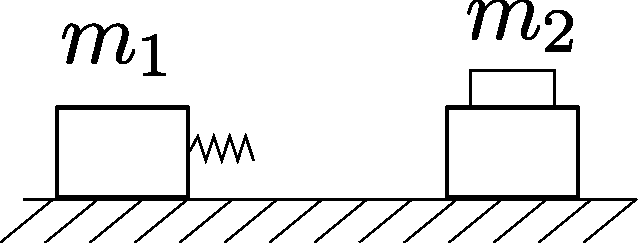
\includegraphics{colisionelastica}
  \caption{Colisión elástica}
  \label{fig:colisionelastica}
\end{figure}

Como la colisión ocurre prácticamente en un punto, podemos despreciar
la energía disipada en calor durante el pequeño intervalo de tiempo
que dura la colisión. Entonces la energía cinética se conserva antes y
después de la colisión. 

Conservación de moméntum
\begin{align}
  \label{eq:e1}
  p_{i}=&p_f\nonumber\\
  m_1 u_1 =& m_1 v_1 + m_2 v_2\,.
\end{align}

Conservación de energía cinética
\begin{align}
  \label{eq:e2}
  K_i=&K_f\nonumber\\
  m_1 u^2_1 =& m_1 v^2_1 + m_2 v^2_2\,.
\end{align}

De (\ref{eq:e1})
\begin{equation}
  \label{eq:v1}
  v_1 = \frac{1}{m_1}( m_1u_1 - m_2 v_2),
\end{equation}
Reemplazando $v_1$ en \ref{eq:e2}
\begin{equation}
   m_1 u_1^2 = m_1 \left( \frac{m_1u_1 - m_2 v_2}{m_1} \right)^2 +  m_2 v^2_2\,,
\end{equation}
y desarrollando el binomio
\begin{align}
 m_1 u_1^2 =& \frac{1}{m_1}( m_1^2 u_1^2 - 2 m_1 m_2 u_1 v_2 + m_2^2 v_2^2) + m_2 v_2^2\nonumber\\
m_1 u_1^2 =&  m_1 u_1^2 - 2 m_2 u_1 v_2 + \frac{m_2^2}{m_1} v_2^2 + m_2 v_2^2\,.
\end{align}
Cancelando $m_1 u_1^2$ a ambos lados y dividiendo por $m_2v_2$ y factorizando $v_2$
\begin{align}
  0=& - 2 m_2 u_1 v_2 + \frac{m_2^2}{m_1} v_2^2 + m_2 v_2^2\nonumber\\
  0=& - 2  u_1  + \frac{m_2}{m_1} v_2 + v_2\nonumber\\
  0=& - 2  u_1  + \left(\frac{m_2}{m_1} +1 \right)v_2\nonumber\\
  0=& - 2  u_1  + \left(\frac{m_2+m_1}{m_1}\right)v_2\,,
\end{align}
obtenemos
\begin{equation}
  v_2 = \frac{2m_1}{m_1+ m_2}u_1\,.
\end{equation}
Reemplazando este valor en \eqref{eq:v1}

\begin{align}
  v_1 =& \frac{1}{m_1}\left(m_1u_1 - \frac{2m_2 m_1u_1}{m_1+m_2} \right)\nonumber\\
  =& \frac{u_1}{m_1}\left(m_1 - \frac{2m_2 m_1}{m_1+m_2} \right)\nonumber\\
  =& u_1\left(1 - \frac{2m_2}{m_1+m_2} \right)\nonumber\\
  =& u_1\left(\frac{m_1+m_2 - 2m_2}{m_1+m_2} \right)\nonumber\\
  v_1 = &\frac{m_1 - m_2}{m_1 + m_2} u_1
\end{align}
Asumiendo que el bloque 1 se mueve inicialmente hacia la derecha: $u_1>0$,  tenemos los siguientes casos:
\begin{align}
  v_1\to
  \begin{cases}
    =0 & \text{si\ }m_1=m_2\\
    >0 & \text{si\ }m_1>m_2\\
    <0 & \text{si\ }m_1<m_2
  \end{cases}\,.
\end{align}
\finejemplo







\subsection{Colisiones inelásticas}
En un segundo experimento, tome el mismo par de bloques y reemplace el
resorte por una masilla adhesiva. Considere el segundo bloque
inicialmente en reposo. Después de la colisión ambos bloques se quedan
pegados y se mueven con alguna velocidad $v'$. Por conservación del
moméntum
\begin{align}
  m_1 v=(m_1+m_2)v'\,,
\end{align}
de modo que
\begin{align}
  v'=\frac{m_1}{m_1+m_2}v\,.
\end{align}
La diferencia de energías cinéticas inicial menos final:
\begin{align}
  \tfrac{1}{2}m_1v^2-\tfrac{1}{2}(m_1+m_2)v'^2=&
  \tfrac{1}{2}m_1v^2-\tfrac{1}{2}(m_1+m_2)\frac{m_1^2}{(m_1+m_2)^2}v^2\nonumber\\
  =&\tfrac{1}{2}m_1v^2-\tfrac{1}{2}\frac{m_1^2}{m_1+m_2}v^2\nonumber\\
  =&\tfrac{1}{2}m_1v^2  \left(1-\frac{m_1}{m_1+m_2} \right)
\end{align}
es claramente diferente de cero. Por ejemplo, si $m_1=m_2$, la energía
disipada corresponde a la mitad de la energía cinética inicial. La
energía cinética a cambiado debido a que las fuerzas fueron no
conservativas. Parte de la energía del movimiento colectivo fue
transformada en una energía calórica en el proceso de pegado durante
la colisión. Una colisión en la cual la energía es no conservada es
llamada una \emph{colisión inelástica}. Si los cuerpos quedan juntos
después de la colisión, decimos que la colisión es completamente
inelástica.


Aunque la energía total del sistema es siempre conservada en colisiones, parte de la energía cinética puede ser convertida a alguna otra forma. Para tener en cuenta éste hecho, escribamos la conservación de la energía para colisiones como
\begin{align}
\label{eq:calor}
  K_i=K_f+Q\,,
\end{align}
donde $Q=K_i-K_f$ es la cantidad de energía cinética convertida a otra forma

Para colisiones en una dimensión, la ec.~\eqref{eq:consmom}
Conservación de moméntum  se reduce a
\begin{equation}\label{eq:E1}
  m_1 v_1 + m_2 v_2 = m_1 v_1' + m_2 v_2'\,,
\end{equation}
y conservación de energía cinética es
\begin{equation}\label{eq:E2}
  m_1 v^2_1 + m_2 v^2_2 = m_1 {v'}^2_1 + m_2 {v'}^2_2+Q\,.
\end{equation}
Una vez se calcule $Q$, el sistema de dos ecuaciones con dos
incógnitas se puede resolver

\ejemplo{}
\begin{frame}[fragile,allowframebreaks]
 \textbf{Colisiones
    inelásticas:}\footnote{Elaborado por Nicolás Moure} Un bloque de masa $m$ inicialmente en reposo
  en el punto $A$, se deja caer por una superficie circular de radio
  $R$ como se muestra en la figura ~\ref{fig:colision}. Al llegar al
  punto $B$, sufre una colisión totalmente inelástica con un segundo
  bloque de la misma masa y se quedan pegados hasta alcanzar el reposo
  en $D$. Las dos secciones circulares, tramos $AB$ y $CD$, son
  completamente lisas. El tramo $BC$ es rugoso y el coeficiente de
  fricción entre los bloques y la superficie del piso es
  $\mu$. Encuentre el  el ángulo $\theta$ mostrado en la figura ~\ref{fig:colision}

  \begin{figure}
    \centering
    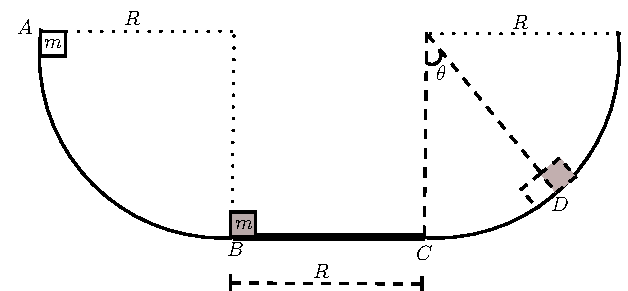
\includegraphics{colision}
    \caption{Ejemplo conservación de energía y colisiones inelásticas}
    \label{fig:colision}
  \end{figure}


\end{frame}

\noindent
\textbf{Solución}] 
En los tramos $AB$ y $CD$ sólo realiza trabajo el peso porque
$\mathbf{N}$ es perpendicular a la trayectoria. En el sector $BC$ sólo
realiza trabajo la fricción, porque el peso y la normal sor
perpendiculares a la trayectoria. El peso es una fuerza conservativa,
mientras que la fricción es una fuerza no conservativa.



En el sector AB: Conservación de la energía
\begin{align}
  mgR=\tfrac{1}{2}m v^2_B\,
\end{align}
de donde
\begin{align}
  v_B=\sqrt{2gR}
\end{align}

En el sector $BC$: El moméntum en la dirección horizontal es igual justo
antes y justo después de la colisión; como la colisión es
completamente inelástica los cuerpos se quedan pegados
\begin{align}
  m v_B=&(m+m) v_B'\nonumber\\
  m v_B=&2m v_B'\nonumber\\
   v_B=&2v_B'\,,
\end{align}
entonces
\begin{align}
  v_B'=&\tfrac{1}{2}v_B\nonumber\\
  =&\tfrac{1}{2}\sqrt{2gR}\nonumber\\
  =&\sqrt{\frac{gR}{2}}\,.
\end{align}
Como la fricción es constante en $BC$,
\begin{align}
  W_f=-f(x_C-x_B)=-f R\,.
\end{align}
Por otro lado $f=\mu N_2=2 m g$, de modo que
\begin{align}
  W_f=-2 \mu m g R=-Q\,.
\end{align}
De la ec.~\eqref{eq:calor}
\begin{align}
  K_B-K_C=Q=2\mu m g R\,.
\end{align}
de donde
\begin{align}
  \tfrac{1}{2}(2m){v_B'}^2-  \tfrac{1}{2}(2m)v_C^2=&2\mu m g R\nonumber\\
  {v_B'}^2- v_C^2=&2\mu  g R
\end{align}
despejando $v_C$
\begin{align}
   v_C^2=&{v_B'}^2-2\mu g R\nonumber\\
\end{align}
\begin{align}
  v_C^2=&\frac{gR}{2}-2\mu g R\nonumber\\
  =&\frac{gR}{2}\left(1-4\mu \right)\,.
\end{align}
de modo que
\begin{align}
  v_C=&\sqrt{\frac{gR}{2}\left(1-4\mu \right)}\,.
\end{align}
El sistema alcanza a llegar a $C$ si $v_c$ es real, esto es si
\begin{align}
  1-4\mu\ge 0\Longrightarrow \mu\le \frac{1}{4}\,.
\end{align}

En el sector CD: Conservación de la energía
\begin{align}
  \tfrac{1}{2}(2m)v_C^2=&2mgh\nonumber\\
&=2mg(R-R\cos\theta)\nonumber\\
&=2mgR(1-\cos\theta)\nonumber\\
  \frac{1}{2}\cdot\frac{gR}{2}\left(1-4\mu \right)&=gR(1-\cos\theta)\nonumber\\
  \frac{1}{4}\left(1-4\mu \right)&=1-\cos\theta\nonumber\\
  \frac{1}{4}-\mu&=1-\cos\theta\,.
\end{align}
\begin{align}
  \cos\theta=&1-\frac{1}{4}+\mu\nonumber\\
  =&\frac{3}{4}+\mu\,,
\end{align}
El $\theta_{\text{min}}$ se obtiene cuando $\mu=1/4$:
\begin{align}
 \cos \theta_{\text{min}}=&1 &\text{o} \qquad \theta_{\text{min}}=0
\end{align}
Así mismo, el $\theta_{\text{max}}$ se obtiene cuando $\mu=0$:
\begin{align}
  \theta_{\text{max}}&\approx 0.723\ \text{rad}\nonumber\\
&\approx 41.4^\circ\,.
\end{align}
Note que si $m=\SI{1}{\kilo\gram}$ y $R=\SI{1}{\meter}$, la energía disipada en
forma de calor en el tramo $BC$ cuando $\mu=0.1$ es
\begin{align}
  Q=&2 \mu m g R\nonumber\\
  =&2\cdot 0.1\cdot \SI{1}{\kilo\gram}\cdot \SI{9.8}{\meter\per\second^2}\cdot
  \SI{1}{\meter}\nonumber\\
  =&\SI{1.96}{\kilo\gram \meter^2\per\second^2}\nonumber\\
  =&\SI{1.96}{\joule}\,.
\end{align}

\finejemplo





\section{Colisiones y coordenadas de centro de masa}
Para estudiar las colisiones de dos partículas que se mueven con
velocidades $\mathbf{v}_1$ y $\mathbf{v}_2$ en lo que se denomina \emph{sistema de
  laboratorio} $L$, es conveniente reescribir las posiciones y velocidades
en el sistema de centro de masa $C$.

Del Capítulo \ref{cha:momentum} sobre moméntum, tenemos:
  \begin{align}
    \label{eq:mbaton}
    \mathbf{R}=\frac{m_1\mathbf{r}_1+m_2\mathbf{r}_2}{m_1+m_2}
  \end{align}
De modo que las coordenadas en el sistema $C$ satisfacen:
\begin{align}
  \mathbf{r}_{1c} =&\mathbf{r}_1-\mathbf{R}\nonumber\\
  \mathbf{r}_{2c}=&\mathbf{r}_2-\mathbf{R}\,.
\end{align}
De la ec.~(\ref{eq:mbaton})
\begin{align}
\label{eq:r12cm}
  \mathbf{r}_{1c}
    =&\frac{m_2}{m_1+m_2}(\mathbf{r}_1-\mathbf{r}_2)\nonumber\\
 \mathbf{r}_{2c}=&-\left(\frac{m_1}{m_1+m_2} \right)\left(\mathbf{r}_1-\mathbf{r}_2 \right)\,.
\end{align}
Derivando con respecto al tiempo estas expresiones, obtenemos
 
\begin{minipage}{0.5\linewidth}
  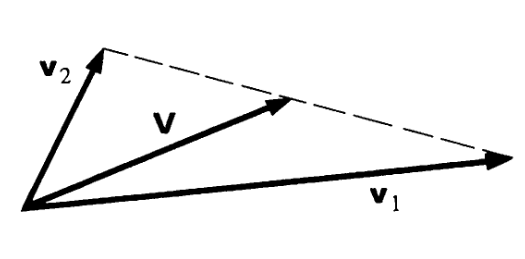
\includegraphics[scale=0.35]{vcm}

\noindent
$V$ está en la línea que une $\mathbf{v}_1$ con $\mathbf{v}_1$.
\end{minipage}
\begin{minipage}{0.5\linewidth}
  \begin{align}
    \label{eq:Vcm}
    \mathbf{V}=\frac{m_1\mathbf{v}_1+m_2\mathbf{v}_2}{m_1+m_2}
  \end{align}
\end{minipage}


\begin{minipage}{0.5\linewidth}
  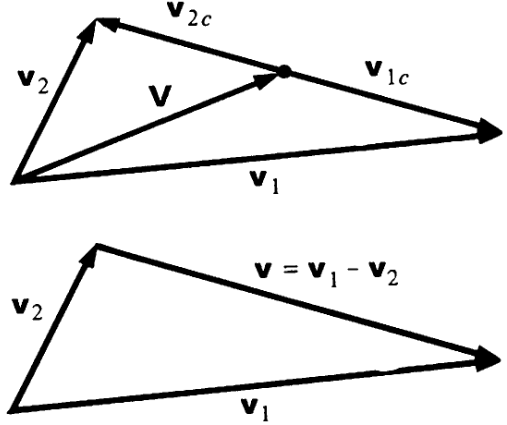
\includegraphics[scale=0.35]{v12cm}

\noindent
$\mathbf{v}_{1c}$ y $\mathbf{v}_{2c}$ están en direcciones opuestas a lo largo del vector de velocidad relativa $\mathbf{v}=\mathbf{v}_1-\mathbf{v}_2$
\end{minipage}
\begin{minipage}{0.5\linewidth}
De modo que las coordenadas en el sistema $C$ satisfacen:
\begin{align}
  \label{eq:v12cm}
  \mathbf{v}_{1c} =&\mathbf{v}_1-\mathbf{V}\nonumber\\
  \mathbf{v}_{2c}=&\mathbf{v}_2-\mathbf{V}\,.
\end{align}
De la ec.~(\ref{eq:r12cm})
\begin{align}
  \label{eq:v12cm12}
  \mathbf{v}_{1c}
    =&\frac{m_2}{m_1+m_2}(\mathbf{v}_1-\mathbf{v}_2)\nonumber\\
 \mathbf{v}_{2c}=&-\left(\frac{m_1}{m_1+m_2} \right)\left(\mathbf{v}_1-\mathbf{v}_2 \right)\,.
\end{align}
\end{minipage}
  
De esta forma, las cantidades de movimiento desde el sistema $C$ son
\begin{align}
  \mathbf{p}_{1c}=&m_1\mathbf{v}_{1c}\nonumber\\
                =&\frac{m_1m_2}{m_1+m_2}(\mathbf{v}_1-\mathbf{v}_2)\nonumber\\
                =&\mu(\mathbf{v}_1-\mathbf{v}_2)\nonumber\\
\end{align}
\begin{align}
    \mathbf{p}_{2c}=&m_2\mathbf{v}_{2c}\nonumber\\
    =&-\left(\frac{m_1m_2}{m_1+m_2} \right)\left(\mathbf{v}_1-\mathbf{v}_2 \right)\nonumber\\
                =&-\mu(\mathbf{v}_1-\mathbf{v}_2)\,,
\end{align}
donde
\begin{align}
  \mu=\frac{m_1m_2}{m_1+m_2}\,.
\end{align}

Podemos ahora calcular el moméntum total en el sistema de centro de masa $C$
\begin{align*}
\mathbf{p}_{1c}+\mathbf{p}_{2c}=&\mu(\mathbf{v}_1-\mathbf{v}_2)
-\mu(\mathbf{v}_1-\mathbf{v}_2)\nonumber\\
=&0\,,
\end{align*}
y las cantidades de movimiento en el centro de masa son iguales y opuestas
\begin{align}
  \mathbf{p}_{1c}=&-\mathbf{p}_{2c}\,.
\end{align}

El moméntum en el sistema $L$ es
\begin{align*}
  m_1\mathbf{v}_1+m_2\mathbf{v}_2=&(m_1+m_2)\frac{m_1\mathbf{v}_1+m_2\mathbf{v}_2}{m_1+m_2}\nonumber\\
  =&(m_1+m_2)\mathbf{V}
\end{align*}
y ya que el moméntum es conservado en cualquier colisión, entonces
$\mathbf{V}$ es constante. 
Podemos usar este resultado como una ayuda para visualizar los
vectores de velocidad antes y después de la colisión.

\begin{figure}
  \centering
  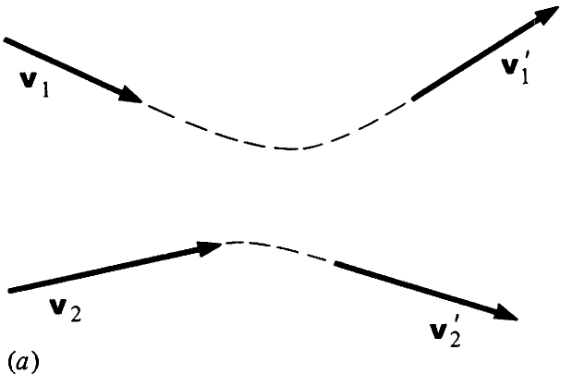
\includegraphics[scale=0.3]{coli1}
  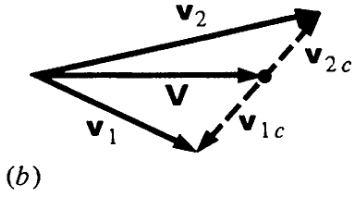
\includegraphics[scale=0.3]{coli2}
  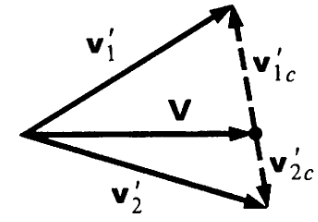
\includegraphics[scale=0.3]{coli3}

\hspace{7cm}{(c)}
  \caption{Colisiones}
  \label{fig:coli}
\end{figure}

La figura~\ref{fig:coli}~(a) muestra las trayectoria y velocidades de
dos partículas en colisión.  
En la figura~\ref{fig:coli}~(b) mostramos las velocidades iniciales en
los sistema $L$ y $C$.
Todos los vectores están sobre el mismo plano.
$\mathbf{v}_{1c}$ y $\mathbf{v}_{2c}$ deben estar espalada con espalda
ya que el moméntum total en el sistema $C$ es cero. 

Después de la colisión, como se muestra en la
figura~\ref{fig:coli}~(c), las velocidades en el sistema $C$ son de
nuevo espalda a espalda.
La figura también muestra las velocidades
finales en el sistema de laboratorio, obtenidas siguiendo el mismo
procedimiento usado para llegar a la ec.~\eqref{eq:v12cm12}. 

Reescribiendo
$\mathbf{V}$ dado por la ec.~(\ref{eq:v12cm}),  en términos de 
las velocidades después de la colisión
  \begin{align}
    \label{eq:Vpcm}
    \mathbf{V}=\frac{m_1\mathbf{v}_1'+m_2\mathbf{v}_2'}{m_1+m_2}
  \end{align}
Repitiendo los mismos pasos pero en términos de las velocidades
finales, tenemos que
\begin{align}
  \label{eq:v12pcm12}
  \mathbf{v}_{1c}'=&\mathbf{v}_1'-\mathbf{V}\nonumber\\
    =&\frac{m_2}{m_1+m_2}(\mathbf{v}_1'-\mathbf{v}_2')\nonumber\\
 \mathbf{v}_{2c}'= &\mathbf{v}_2'-\mathbf{V}\nonumber\\
=&-\left(\frac{m_1}{m_1+m_2} \right)\left(\mathbf{v}_1'-\mathbf{v}_2' \right)\,.
\end{align}


Note que el plano de la figura~\ref{fig:coli}~(c) no es necesariamente
el plano de la figura~\ref{fig:coli}~(a). 
Evidentemente las relaciones geométricas entre las velocidades
iniciales y finales en el sistema $L$ es bastante complicado. 
Afortunadamente, la situación en el sistema $C$ es mucho más simple. 
Las velocidades iniciales y finales en el sistema $C$ determinan un
plano conocido como el plano de dispersión. 
Cada partícula es desviada a través del mismo ángulo de dispersión
$\Theta$ en este plano.

La fuerza de interacción debe ser conocida para poder calcular
$\Theta$, o al contrario, midiendo la desviación podemos aprender
sobre la fuerza de interacción. Sin, embargo evitaremos estas
consideraciones y asumiremos que la interacción ha causado alguna
desviación en el sistema $C$.


Si además la colisión es elástica y denotando con primas las
velocidades después de la colisión tenemos
\begin{align}
\label{eq:cecm}
  \tfrac{1}{2}m_1 v_{1c}^2+  \tfrac{1}{2}m_2 v_{2c}^2
= \tfrac{1}{2}m_1 {v_{1c}'}^2+ \tfrac{1}{2}m_2 {v_{2c}'}^2\,.
\end{align}
Ya que el moméntum inicial y final es cero, y escogiendo
convenientemente el eje $x$ de los sistemas $C$ y $C$, de manera que
coincida con los vectores moméntum, tenemos
\begin{align}
  m_1 v_{1c}+m_2 v_{2c}=&0 \nonumber\\
  m_2 v_{1c}'+m_2 v_{2c}'=&0\,
\end{align}
y
\begin{align}
\label{eq:ccp}
  v_{2c}=&-\frac{m_1}{m_2}v_{1c}\nonumber\\
  v_{2c}'=&-\frac{m_1}{m_2}v_{1c}'\,.
\end{align}
Reemplazando en ec.~(\ref{eq:cecm})
\begin{align}
  m_1 v_{1c}^2+  \frac{m_1^2}{m_2} v_{1c}^2
=& m_1 {v_{1c}'}^2+ \frac{m_1^2}{m_2} {v_{1c}'}^2 \nonumber\\
 \left(m_1+\frac{m_1^2}{m_2}  \right) v_{1c}^2
=&\left(m_1+\frac{m_1^2}{m_2}  \right) {v_{1c}'}^2 \nonumber\\
v_{1c}^2=&{v_{1c}'}^2\,,
\end{align}
de modo que
\begin{align*}
  v_{1c}=&v_{1c}'\,.
\end{align*}
Sustituyendo en la ec.~(\ref{eq:ccp}), obtenemos que
\begin{align*}
  v_{2c}=&v_{2c}'\,.
\end{align*}
En resumen, el problema general de lo colisión de dos cuerpos, visto
desde el sistema del centro de masa, implica que
\begin{align}
  v_{1c}=&v_{1c}'\nonumber\\
  v_{2c}=&v_{2c}'\,.
\end{align}
En una colisión elástica, la rapidez de cada partícula en el sistema
de centro de masa es la misma antes y después de la colisión. Así, los
vectores de velocidad simplemente rotan en el ángulo de dispersión,
como se muestra en la figura~\ref{fig:particolgen}
\begin{figure}
  \centering
  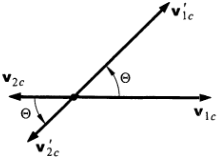
\includegraphics[scale=0.6]{particolgen}
  \caption{Colisión general de dos cuerpos}
  \label{fig:particolgen}
\end{figure}


\subsection{Ángulo de dispersión}
Considere la dispersión elástica de una partícula de masa $m_1$ y
velocidad $\mathbf{v}_1$ con una partícula de masa $m_2$ en reposo,
como se muestra en la figura~\ref{fig:collitarget} (a). 
Después de la colisión las partículas se mueven con velocidades
$\mathbf{v}_1'$ y $\mathbf{v}_2'$.
Es más fácil analizar el movimiento desde el Sistema de centro de
masa. 
Como no hay fuerzas externas actuando sobre el par de partículas, el
centro de masa se mueve a velocidad constante [ver
fig.~\ref{fig:collitarget}~(c)] dada por la ec.~(\ref{eq:Vcm}) con
$\mathbf{v}_2=0$
\begin{align}
  \label{eq:Vv20}
  \mathbf{V}=\frac{m_1}{m_1+m_2}\mathbf{v}_1\,.
\end{align}
Un observador en el centro de masa ve las dos partículas moverse con
la velocidades dadas en la ec.~\eqref{eq:v12cm}
\begin{align*}
  \mathbf{v}_{1c} =&\mathbf{v}_1-\mathbf{V}\nonumber\\
  \mathbf{v}_{2c}=&-\mathbf{V}\,,
\end{align*}
e ilustradas en la fig.~\ref{fig:collitarget}~(d). De las ecuaciones~\eqref{eq:v12cm12}
\begin{align}
  \label{eq:v12cm12v20}
  \mathbf{v}_{1c}
    =&\frac{m_2}{m_1+m_2}\mathbf{v}_1\nonumber\\
 \mathbf{v}_{2c}=&-\frac{m_1}{m_1+m_2}\mathbf{v}_1\,.
\end{align}


Como después de la colisión la velocidad $\mathbf{v}_2'$ es diferente
de cero, entonces
\begin{align}
  \label{eq:v12c}
  \mathbf{v}_{1c}' =&\mathbf{v}_1'-\mathbf{V}\nonumber\\
  \mathbf{v}_{2c}'=&\mathbf{v}_2'-\mathbf{V}\,.
\end{align}

\begin{frame}
\begin{figure}
  \centering
%\only<1>%
{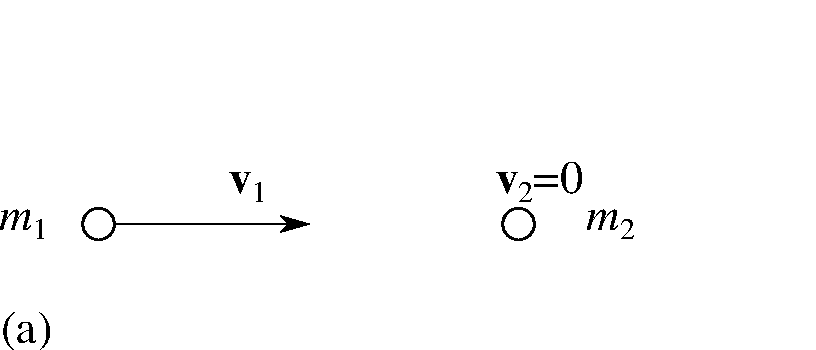
\includegraphics[scale=0.6]{collitargeta}}
%\only<2>%
{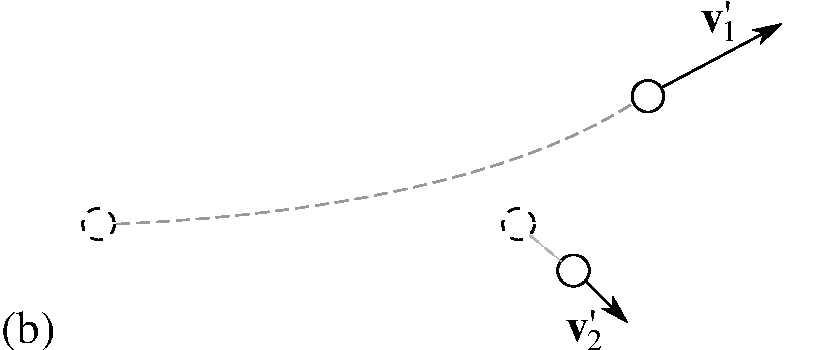
\includegraphics[scale=0.6]{collitargetb}}\nobreakinbeamer
%\only<3>%
{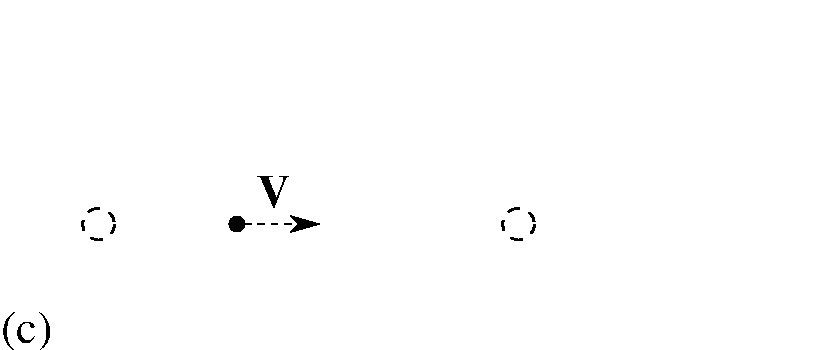
\includegraphics[scale=0.6]{collitargetc}}
%\only<4>%
{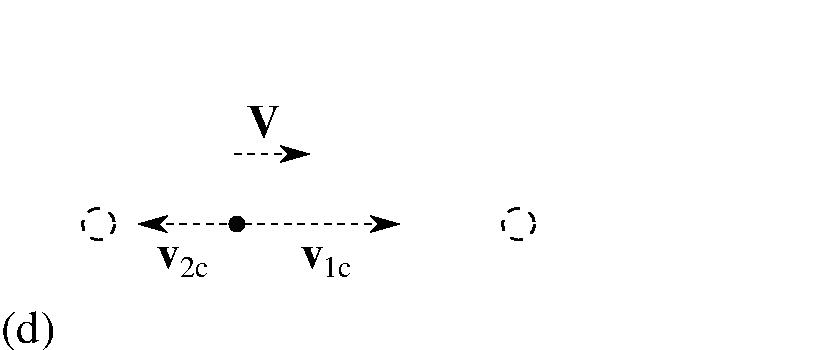
\includegraphics[scale=0.6]{collitargetd}}\nobreakinbeamer
%\only<5>%
{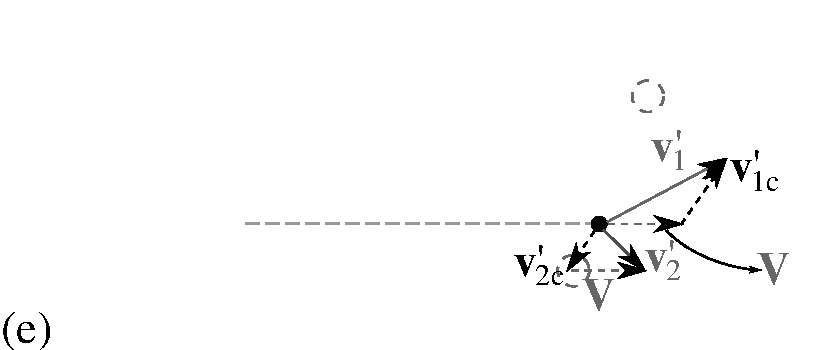
\includegraphics[scale=0.6]{collitargete}}
%\only<6>%
{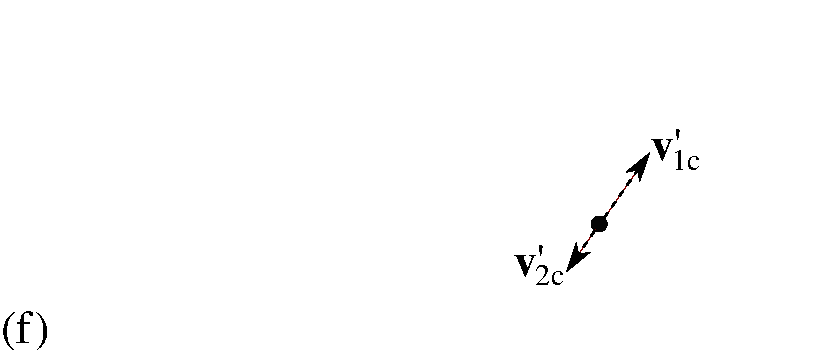
\includegraphics[scale=0.6]{collitargetf}}
  \caption{Colisión con blanco en reposo}
  \label{fig:collitarget}
\end{figure}
\end{frame}

Estas sumas vectoriales están representadas en la
fig.~\ref{fig:collitarget}~(e) que dan lugar a los vectores espalda a
espalda mostrados en la fig.~\ref{fig:collitarget}~(e), con
$\mathbf{v}_{1c}'$, por ejemplo, formando un ángulo $\Theta$ con la
dirección de $\mathbf{v}_{1c}$ como se representa en la figura~\ref{fig:collitargetg}. 

Allí tenemos de nuevo la representación geométrica de la ecuación para
$\mathbf{v}_{1c}'$ dada por la ec.~\eqref{eq:v12c}.

\begin{frame}
\begin{figure}
  \centering
  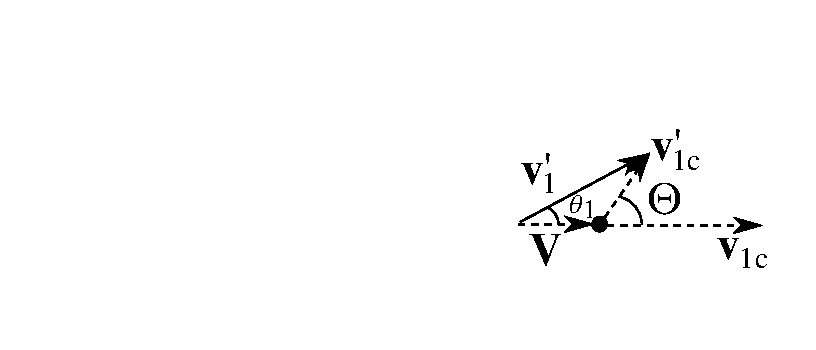
\includegraphics[scale=0.8]{collitargetg}
  \caption{Ángulo de dispersión}
  \label{fig:collitargetg}
\end{figure}
\end{frame}

El ángulo $\Theta$ puede variar en todo su rango desde $0$ hasta
$2\pi$. Para hallar la relación con uno de los ángulo en el sistema de
laboratorio, $\theta_1$, tenemos de la trigonometría de la
fig.~\ref{fig:collitargetg} que
\begin{align}
  \tan\theta_1=&\frac{v_{1c}'\sin\Theta}{V+v_{1c}'\cos\Theta}\nonumber\\
  =&\frac{\sin\Theta}{\left(V/v_{1c}'\right)V+\cos\Theta}\,.
\end{align}

Ya que $v_{1c}'=v_{1c}$
\begin{align}
  \label{eq:tanth1}
  \tan\theta_1=&\frac{\sin\Theta}{\left(V/v_{1c}\right)V+\cos\Theta}\,.
\end{align}

Desarrollando la magnitud del vector $\mathbf{v}_{1c}$ en las
ecs.~\eqref{eq:v12cm12v20}, 
\begin{align*}
 v_{1c}=&\frac{m_2}{m_1+m_2}v_1\,, 
 \end{align*}
y usando la ec.~\eqref{eq:Vv20}, tenemos
\begin{align*}
  v_{1c}=&\frac{m_2}{m_1}\frac{m_1}{m_1+m_2}v_1\nonumber\\
  =&\frac{m_2}{m_1}V\,.
\end{align*}
De modo que
\begin{align*}
  \frac{V}{v_{1c}}=\frac{m_1}{m_2}.
\end{align*}
Reemplazando finalmente en~\eqref{eq:tanth1}, tenemos finalmente que
\begin{align*}
    \tan\theta_1=&\frac{\sin\Theta}{\left(m_1/m_2\right)+\cos\Theta}\,.
\end{align*}
Cuando $m_1/m_2<1$ (o $m_1<m_2$), $\theta_1$ también puede variar entre $0$ y
$2\pi$. Pero si $m_1>m_2$, $\tan\theta_1$ queda limitado por un valor
máximo. En particular en el límite en $m_1>>m_2$:
\begin{align*}
  \tan\theta_1\approx \frac{m_2}{m_1}\tan\Theta\to 0\qquad\text{si $m_1>>m_2$}\,.
\end{align*}
Una bola muy pesada simplemente arrastra la pequeña pero sin cambiar
sustancialmente la dirección.




\section{Problemas resueltos}
\begin{enumerate}
\item Un auto \textbf{A} cuya rapidez es $v_1$ choca con un auto \textbf{B}, cuya rapidez es $v_2$, tal como se muestra en la figura. La masa del auto \textbf{A} es $m$ y la masa del auto \textbf{B} es $6/5$ $m$. Se sabe que los automóviles se aproximaban con cantidads de movimiento de igual magnitud y direcciones opuestas, y que la colisión es elástica, es decir, que la energía cinética del sistema se conserva en la colisión.

  \begin{minipage}{0.4\linewidth}
    \includegraphics[scale=0.7]{colision1}    
  \end{minipage}  \begin{minipage}{0.6\linewidth}
    \begin{enumerate}
    \item Determine  $v_2$ en términos de $v_1$.% y  v'2 en términos de  v'1 .
      \label{item:p1a}
    \item Encuentre la magnitud de las velocidades $v'_1$ y $v'_2$ de cada auto después de la colisión.
      \label{item:p1b}
    \item Calcule las cantidades del literal anterior para  $v_1=10$ m/s. 
      \label{item:p1c}
    \end{enumerate}
  \end{minipage}
\begin{itemize}
\item[\textbf{Solución:}]
  \begin{itemize}
  \item[\ref{item:p1a}]: De la conservación del moméntum, sobe la línea de colisión
    \begin{align*}
      \mathbf{p}_1+\mathbf{p}_2=&0\nonumber\\
      m v_1-\tfrac{6}{5}m v_2=&0\nonumber\\
      v_2=\tfrac{5}{6}v_1
    \end{align*}
  \item[~\ref{item:p1b}]
    El momentúm después de la colisión es cero y por consiguiente
\begin{align*}
  v_2'=\tfrac{5}{6}v_1'\,,
\end{align*}
De la conservación de energía cinética
\begin{align*}
  \tfrac{1}{2}m v_1^2+\tfrac{1}{2}(\tfrac{6}{5}m)  v_2^2=&
  \tfrac{1}{2}m {v_1'}^2+\tfrac{1}{2}(\tfrac{6}{5}m)  {v_2'}^2\nonumber\\
  v_1^2+(\tfrac{5}{6})  v_1^2=&
  {v_1'}^2+(\tfrac{5}{6}) {v_1'}^2\nonumber\\
  \frac{11}{6}{v_1^2}'=&\frac{11}{6}v_1^2\nonumber\\
  {v_1^2}'=&v_1^2\,,
\end{align*}
y entonces
\begin{align*}
 v_2'=\tfrac{5}{6}v_1\,.
\end{align*}

  \end{itemize}

\end{itemize}


\item 

\item (Tomado de \cite{gabriel}) Un bloque de masa $m$ se suelta desde el punto $A$ y este se desliza sobre el cuadrante circular $AB$ de radio $R$, llegando a $B$ con velocidad $v_1$ de acuerdo a la figura. En $B$ choca elásticamente con el bloque de masa $2m$ que se encuentra inicialmente en reposo. Luego del choque, la masa $2m$ se mueve sobre la superficie horizontal lisa hasta chocar y comprimir un resorte de constante elástica $k$. El cuadrante circular AB es rugoso. Calcular

  \begin{minipage}{0.5\linewidth}
    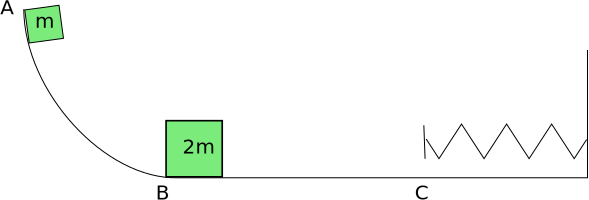
\includegraphics[scale=0.5]{planosuple}
  \end{minipage}
  \begin{minipage}{0.5\linewidth}
    \begin{enumerate}
    \item El trabajo realizado por la fuerza de fricción en el tramo $AB$.
      \label{item:p2a}
    \item La velocidad de cada bloque después del choque.
      \label{item:p2b}
    \item La compresión del resorte.
      \label{item:p2c}
    \item Calcule las cantidades de los literales anteriores para $m=2\ $Kg, $RO=0.5\ $m, $v_1=2.1\ $m/s, $k=1000\ $N/m
    \end{enumerate}
  \end{minipage}

%sln pag 130
  \begin{itemize}
  \item[\textbf{Solución}]
  \item[\ref{item:p2a}]
    \begin{align*}
      W_{ba}=&E_b-E_a\nonumber\\
      =&\tfrac{1}{2}m v_1^2-mgR\,,
    \end{align*}
  \item[\ref{item:p2b}] 
    \begin{align}
      \label{eq:pp2b}
      m v_1=&m v_1'+2m v_2'\\
      \label{eq:pp2bb}
      \tfrac{1}{2}m v_1^2=&\tfrac{1}{2}m {v_1'}^2+\tfrac{1}{2}(2m){v_2'}^2\,.
    \end{align}
    de \eqref{eq:pp2b}
    \begin{align*}
      v_1'=v_1-2v_2'\,,
    \end{align*}
    y en \eqref{eq:pp2bb}
    \begin{align*}
      2{v_2'}^2=&v_1^2-{v_1'}^2\nonumber\\
      =&v_1^2-(v_1^2-4 v_1 v_2'+4{v_2'}^2)\nonumber\\
      =&4v_2'(v_1-v_2')\,.
    \end{align*}
    Simplificando
    \begin{align*}
      v_2'=2v_1-2v_2'\,,
    \end{align*}
    y
    \begin{align*}
      v_2'=\tfrac{2}{3}v_1\,,
    \end{align*}
    además
    \begin{align*}
      v_1'=&v_1-2v_2'\nonumber\\
      =&v_1-\tfrac{4}{3}v_1\nonumber\\
      =&-\tfrac{1}{3}v_1\nonumber\\
    \end{align*}
  \item[\ref{item:p2c}]
    \begin{align*}
      \tfrac{1}{2}(2m){v_2'}^2=&\tfrac{1}{2}kx^2\nonumber\\
       m{v_2'}^2=&\tfrac{1}{2}kx^2\nonumber\\
       mv_2'=&\tfrac{1}{2}\sqrt{k}x\nonumber\\
    \end{align*}
    \begin{align*}
      x=&{v_2'}\sqrt{\frac{2m}{k}}\nonumber\\
      =&\frac{2v_1}{3}\sqrt{\frac{2m}{k}}\,.
    \end{align*}
  \end{itemize}


\item Un anillo resbala a lo largo de un arco metalico ABC muy pulido
  que es arco de una circunferencia de radio
  $R=\SI{1.2}{\meter}$. 
  Sobre el anillo actúa una fuerza $\mathbf{F}$ de magnitud
  $\SI{150}{\newton}$ y dirección constante formando un ángulo de
  $\alpha=\pi/6$ con la horizontal.

  \begin{minipage}{0.5\linewidth}
   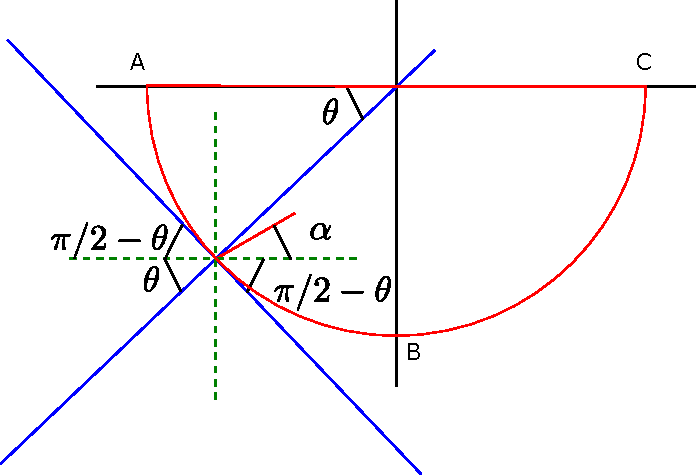
\includegraphics[scale=0.5]{anillos}
  \end{minipage}
  \begin{minipage}{0.5\linewidth}
    Calcular el trabajo efectuado por la fuerza $\mathbf{F}$ sobre el anillo al moverse desde $A$ a $B$ y de $B$ a $C$
  \end{minipage}
  \begin{itemize}
  \item[\textbf{Solución}]
    En la figura se muestra el anillo en una posición general, de la figure tenemos que en el sistema de coordenadas $\hat{\mathbf{r}}$-$\hat{\boldsymbol{\theta}}$:
    \begin{align*}
      \mathbf{F}=F_r \hat{\mathbf{r}}+F_\theta\hat{\boldsymbol{\theta}}\,,
    \end{align*}
    donde
    \begin{align*}
      F_\theta=&F\cos(\pi/2-\theta+\alpha)\nonumber\\
      =&F\sin(\alpha-\theta)\,. %comprobar
    \end{align*}

    Además del próximo capítulo:
    \begin{align*}
      \frac{d\mathbf{r}}{dt}=\frac{dr}{dt} \hat{\mathbf{r}}+ r\frac{d\theta}{dt}\hat{\boldsymbol{\theta}}\,,
    \end{align*}
    de modo que
    \begin{align*}
      d\mathbf{r}=dr \hat{\mathbf{r}}+ r \, d\theta\hat{\boldsymbol{\theta}}\,.
    \end{align*}
    Por la simetría del problema el trabajo para ir de $A$ a $C$ es el doble de ir de $A$ a $B$, además, como el movimiento sólo de da a lo largo de dirección tangencail al arco, entonces sólo la componente tangencial de la fuerza realiza trabajo. Con todas estas consideraciones tenemos:
    \begin{align*}
      W_{AC}=2W_{AB}=&\int_A^B \mathbf{F}\cdot d\mathbf{r}\nonumber\\
      =&2\int_A^B (F_r\hat{\mathbf{r}}+F_\theta\hat{\boldsymbol{\theta}})\cdot (dr \hat{\mathbf{r}}+ r \, d\theta\hat{\boldsymbol{\theta}})\nonumber\\
      =&2\int_A^B (F_\theta r \, d\theta)\hat{\boldsymbol{\theta}}\cdot\hat{\boldsymbol{\theta}}\nonumber\\
      =&2\int_{0}^{\pi/2}F_\theta r \, d\theta\nonumber\\
      =&2Fr\int_{0}^{\pi/2}\sin(\alpha-\theta) \, d\theta\nonumber\\
      =&2Fr\cos(\alpha-\theta)|_0^{\pi/2}\nonumber\\
      =&2Fr[\sin(\alpha-\pi/2)-\sin(\pi/6)]\nonumber\\
      =&\SI{131.77}{\joule}\,.
    \end{align*}

   
  \end{itemize}



\item ...
  \begin{minipage}{0.5\linewidth}
    ...
  \end{minipage}
  \begin{minipage}{0.5\linewidth}
    ...
  \end{minipage}
  \begin{itemize}
  \item[\textbf{Solución}]
  \item[iref]
  \end{itemize}
\end{enumerate}

%%% Local Variables: 
%%% mode: latex
%%% TeX-master: "mecanica"
%%% End: 
